%%%%%%%%%%%%%%%%%%%%%%%%%%%%%%%%
%
%
%  Classifying Quaternion Identities
%  and Pythagorean Quintuples and Quaternions
%  (journal article)
%  
%  by Theodore Ehrenborg
%
%
% 
% Last edited: June 27, 2019
%
%
%%%%%%%%%%%%%%%%%%%%%%%%%%%%%%%%%
%
%%%%%%%%%%%%%%%%%%%%%%%%%%%%%%%%%



%%%%%%%%%%%%%%%%%%%%%%%%%%%%%%%%%
%
% pdf settings
%
%%%%%%%%%%%%%%%%%%%%%%%%%%%%%%%%%
%
\pdfpagewidth=8.5truein
\pdfpageheight=11truein





%
%%%%%%%%%%%%%%%%%%%%%%%%%%%%%%%%%



\documentclass[12pt,table]{article}
%\usepackage{anyfontsize}
\usepackage{amssymb, amsmath, fullpage, amsthm}
\usepackage{mathrsfs}
\usepackage{tikz}
\usepackage[title]{appendix}
\usepackage{mathrsfs}
\usepackage{ gensymb }
\usepackage{enumerate}
\usepackage{caption}
\usepackage{comment}
\usepackage{xcolor}
\usepackage{diagbox}
\usepackage[colorinlistoftodos]{todonotes}




\usetikzlibrary{math}
















\parskip2mm

\newtheorem{theorem}{Theorem}[section]
\newtheorem{hypothesis}[theorem]{Hypothesis}
\newtheorem{lemma}[theorem]{Lemma}
\newtheorem{proposition}[theorem]{Proposition}
\newtheorem{corollary}[theorem]{Corollary}
\newtheorem{conjecture}[theorem]{Conjecture}


\theoremstyle{definition}
\newtheorem{definition}[theorem]{Definition}
\newtheorem{example}[theorem]{Example}

\theoremstyle{remark}
\newtheorem{remark}[theorem]{Remark}
\newtheorem{remarks}[theorem]{Remarks}





\hyphenation{Hurwitz}

\font\german = eufm10 scaled\magstep1
\font\Cp = msbm10

\newcommand{\Ccc}{\mathbb C}
\newcommand{\Fff}{\mathbb F}
\newcommand{\Hhh}{\mathbb H}
\newcommand{\Nnn}{\mathbb N}
\newcommand{\Rrr}{\mathbb R}
\newcommand{\Sss}{\mathbb S}
\newcommand{\Zzz}{\mathbb Z}
\newcommand{\Lll}{\mathbb L}
\renewcommand{\Bbb}{\mathbb B}
\newcommand{\Ooo}{\mathbb O}
\newcommand{\Qqq}{\mathbb Q}


\newcommand{\vanish}[1]{}
\newcommand{\coveredby}{\prec}
\newcommand{\divides}{\mid}
\newcommand{\notdivides}{\nmid}
\newcommand{\timesdots}{\times \cdots \times}
\newcommand{\ascodd}{\asc_{\odd}}
\newcommand{\doubleprime}{\prime\prime}
\newcommand{\myfrac}[2]{#1 / #2}
\newcommand{\SSSS}{\mathfrak{S}}
\newcommand{\Gaussian}[2]{\genfrac{[}{]}{0pt}{}{#1}{#2}_q}
\newcommand{\fix}[1]{\todo[inline]{#1}}






\numberwithin{equation}{section}
%\usepackage[bindingoffset=0.2in,
%            left=1in,right=1in,top=1in,bottom=1in,
%            footskip=.25in]{geometry}%Sets margins
%\pagenumbering{gobble}%No page numbers




 


\DeclareMathOperator{\inv}{inv}
\DeclareMathOperator{\frst}{frst}
\DeclareMathOperator{\er}{er}
\DeclareMathOperator{\asc}{asc}
\DeclareMathOperator{\odd}{odd}
\DeclareMathOperator{\Imag}{Im}
\DeclareMathOperator{\Real}{Re}
\DeclareMathOperator{\N}{N}





\begin{document}
%\begin{landscape}


\title{Classifying Quaternion Identities,
Pythagorean Quintuples and Quaternions}


\author{\sc Theodore EHRENBORG
\fix{I should thank Professor Leep.}
%\thanks{
%Corresponding author:
%Department of Mathematics,
%University of Kentucky,
%Lexington, KY 40506-0027,
%USA,
%{\tt theodore.ehrenborg@gmail.com}.}
%\:\: 
%\:\:
}



\date{}
%%%\date{Last edited on \today}

\maketitle



\begin{abstract}
This paper, which is in number theory, explores 
the  
connections between quaternions and primitive Pythagorean quintuples. 
It is known that the square of a Gaussian integer
(a complex number) is a Pythagorean triple $a^2 + b^2 = c^2$.
Less is 
known about the relationship between quaternions, an extension 
of complex numbers, and Pythagorean quintuples
$a^2 + b^2 + c^2 + d^2 = e^2$.
We show that squaring a quaternion produces a subfamily
of Pythagorean quintuples.
Motivated by Conway and Smith's unique
factorization theorem for the
Hurwitz integers,
we present a more general version of
squaring a quaternion which
generates a larger subfamily of Pythagorean quintuples.
Using a counting argument and Jacobi's Four Square Theorem,
we show that unlike the characterization for Pythagorean triples,
the preceding characterization for Pythagorean quintuples is sparse.
Finally, we use a geometric approach to 
characterize 
all Pythagorean
quintuples.
We notice a similarity between the geometric approach
and the quaternion squaring approach in that they
differ by a geometrically defined constant.
\fix{Combine}

This number theory project investigates identities found by
multiplying together quaternions in $ \Lll[x,y,z,w] $, the
Lipschitz quaternions $ \Lll $ adjoined with the
indeterminates $x$, $y$, $z$, $w$.  Recall that quaternions
are $4$-dimensional complex numbers.  These identities provide
solutions to $ \sum_{j = 1}^{p} \tau_j ^ 2 = \left( \sum_{i = 1}^{m}
x_i ^ 2 \right) ^ n $. We present a rigorous definition that captures
the intuitive notion of when two such identities are equivalent. This
definition implies that the true structure of this problem involves the
group action of the direct product $ \mathfrak{S}_4^\pm \times \mathfrak{S}_4^\pm $.  Using
two complementary methods, we compute the number of equivalence
classes for $n = 1, 2, 3, 4,$ where $n$ is the number of
quaternion factors. We move to the case concerning products of complex
numbers, namely $ \Zzz[i][x,y] $. Using the fact that the
Gaussian integers are commutative under multiplication, we
characterize these equivalence classes, thus also providing an
enumeration.
This enumeration quickly gives a proof that
the total number of solutions in $\Zzz[x,y] $
to $a^2 + b^2 = (x^2 + y^2)^n$
is $4n + 4$.
Assuming that all identities when $p = m = 4$
are a product of quaternions, we prove
that
the total number of solutions in $\Zzz[x,y,z,w] $
to $a^2 + b^2 + c^2 + d^2 = (x^2 + y^2 + z^2 + w^2)^n$
is no more than
$ 8 \sum_{i = 0}^n{47^n} $.
Experimental data for $n = 0,1,2,3$
suggests that this expression
is exact.

\end{abstract}

\listoftodos


\section{Pythagorean Triples}




Recall nonnegative integers $a$, $b$ and $c$ are called a
{\em Pythagorean triple} if
\[
    a^2 + b^2 = c^2.
\]
Furthermore, a {\em primitive Pythagorean triple}
is one where $\gcd(a,b,c) = 1$, that is,
$a$, $b$, and~$c$ have  no common factor greater than $1$.
Pythagorean triples have the geometric interpretation that
they are the side lengths of a right triangle having integer
side lengths.




The following theorem characterizes primitive Pythagorean triples.
It was known by Diophantus~\cite[Page 93]{Heath} and
probably discovered by Euclid~\cite{Euclid}.




A proof can be found in Hardy and Wright's book; 
see~\cite[XIII, 13.2]{Hardy_and_Wright}.



\vanish{
Also see page 295 of Heath for
Fermat's area of triangle result.}



\begin{theorem}
Given a primitive
Pythagorean triple $(a,b,c)$, there are integers
$x$ and $y$ such that $0 < y < x$, 
the integers
$x$ and $y$ are of opposite parity,
and
$\gcd(x,y) = 1$
so that
\begin{equation}
\label{equation_primitive_Pythagorean_triple}
     a = x^2-y^2, \:\:\:\: 
     b = 2xy, \mbox{  and  } \:\: c=x^2+y^2.
\end{equation}
\end{theorem}


\begin{example}
{\rm
For instance, 
for
$a = 5$, $b = 12$, and $c = 13$,
we have
$x = 3$
and $y = 2$.
Geometrically this gives the primitive Pythagorean triple
$(5, 12, 13)$ corresponding to the 
$5$-$12$-$13$ right triangle. 
}
\end{example}



\begin{figure}
\begin{center}
\begin{tabular}{ c|c|c|c|c|c } 

 $x$ & $y$ & $x^2 - y^2$ & $2xy$ & $x^2 - y^2$ & Check \\  
 \hline
 $1$ & $0$ & $1$ & $0$ & $1$ & $1^2 + 0^2 = 1^2$ \\  
 $2$ & $1$ & $3$ & $4$ & $5$ & $3^2 + 4^2 = 5^2$ \\  
 $3$ & $2$ & $5$ & $12$ & $13$ & $5^2 + 12^2 = 13^2$ \\  
 $3$ & $1$ & $8$ & $6$ & $10$ & $8^2 + 6^2 = 10^2$ \\  
 $4$ & $1$ & $15$ & $8$ & $17$ & $15^2 + 8^2 = 17^2$ \\  
 $4$ & $2$ & $12$ & $16$ & $20$ & $12^2 + 16^2 = 20^2$ \\  
 $4$ & $3$ & $7$ & $24$ & $25$ & $7^2 + 24^2 = 25^2$ \\  
\end{tabular}
\caption{Generating pairs for Pythagorean triples where
$0 \leq y < x \leq 4$.}
\end{center}
\label{figure_triples}
\end{figure}







There is a well-known connection between primitive Pythagorean triples
and complex numbers. Consider any {\em Gaussian integer} $x+yi$,
where $x, y \in \Zzz$.
If $x + yi$  is squared, the real and imaginary
parts of the resulting Gaussian integer make up two legs of
a Pythagorean triangle as follows. 


\begin{theorem}
Any primitive Pythagorean triple $(a,b,c)$ with
$a^2 + b^2 = c^2$, can be represented
by the square of a Gaussian integer, $x+yi$,
that is,
\[
    a =  \Re{(x+yi)^2},  \:\:\: b = \Im{(x+yi)^2},
    \mbox{   and   }
    c = |(x+yi)^2|,
\]
where $\Re$ and $\Im$ denote the real and imaginary parts of a complex number
and
$| \cdot |$ denotes the modulus of a complex number.
\end{theorem}



Of course, this fact can be proved with
algebra, but a more intuitive 
idea of a proof relies on the definition 
of multiplication. That is, the number $x+yi$ has a modulus, or     
distance from the origin, of $\sqrt{x^2+y^2}$. The modulus of the       
product of two complex numbers is the same as the product of
the moduli of the numbers.
So $(x+yi)^2$ has a modulus of $x^2+y^2$. Thus, the square of a 
Gaussian integer has integer coordinates and an integer distance
from the origin, giving a right triangle with integer sides.
See Figures~\ref{figure_Pythagorean} 
and~\ref{figure_Pythagorean_squared} for diagrams of this 
concept.

\begin{figure}
\begin{center}
\begin{tikzpicture}


\draw[thick,->] (0,0) -- (8,0); 
\draw[thick,->] (0,0) -- (0,4.5);
\draw[thick,->] (0,0) -- (-2.5,0); 
\draw[thick,->] (0,0) -- (0,-2.5);
\draw[dashed] (6,0) -- (6,2);
\fill (6,2) circle (.1cm);
\draw (0,0) -- (6,2) node[anchor=south west] {$x+yi$};
\draw (4.5,1.5) node[anchor=south east] { $\sqrt{x^2 + y^2}$};
\draw (6,1) node[anchor=west] {$y$};
\draw (3,0) node[anchor=north] {$x$};
\end{tikzpicture}
\end{center}
\caption{Geometric representation of a Gaussian integer.}
\label{figure_Pythagorean}
\end{figure}





\begin{figure}
\begin{center}
\begin{tikzpicture}


\draw[thick,->] (0,0) -- (8,0); 
\draw[thick,->] (0,0) -- (0,4.5);
\draw[thick,->] (0,0) -- (-2.5,0); 
\draw[thick,->] (0,0) -- (0,-2.5);
\draw[dashed] (5,0) -- (5,4);
\fill (5,4) circle (.1cm);
\draw (0,0) -- (5,4) node[anchor=south west] {$(x+yi)^2$};
\draw (3.5,2.6) node[anchor=south east ] {$x^2 + y^2$};
\draw (5,2) node[anchor=west] {$2xy$};
\draw (2.5,0) node[anchor=north] {$x^2-y^2$};


\end{tikzpicture}
\end{center}
\caption{A Gaussian integer $x+yi$ after squaring.}
\label{figure_Pythagorean_squared}
\end{figure}

\section{Pythagorean Quintuples via Squaring Quaternions}


Consider the system of quaternions, discovered by Sir William Hamilton 
in 1843~\cite{Hamilton}.
The quaternions can be thought
of as complex numbers extended to four dimensions.
The general
 form of a quaternion is $x+yi+zj+wk$,
where $x, y, z, w \in \Rrr$.
Up to a sign they have $4$ units: $1$, $i$, $j$, and $k$. Their most striking
property is that multiplication is not commutative. 
For example, $i*j = k \neq j*i = -k$.
See Figure~\ref{figure_multiplication_table} 
for the multiplication table of the
quaternions.


\begin{definition}
The {\em modulus} 
of a quaternion
$q =  x+yi+zj+wk$
is given by 
\[
   |q| = \sqrt{x^2 + y^2 + z^2 + w^2}.
\]
The {\em norm} of a quaternion is the modulus squared, that is,
\[
     N =  N(q) = x^2 + y^2 + z^2 + w^2.
\]
\end{definition}


It is straightforward to check the following property.
\begin{lemma}
\label{lemma_norm_multiplicative}
For two quaternions $q_1$ and $q_2$
\[
     N(q_1 \cdot q_2) = N(q_1) \cdot N(q_2).
\]
\end{lemma}



\begin{figure}
\begin{center}
\begin{tabular}{c||c|c|c|c}
$\cdot$ & $1$ & $i$ & $j$ & $k$ \\
\hline
\hline
$1$ & $1$ & $i$ & $j$ & $k$ \\
\hline
$i$ & $i$ & $-1$ & $k$ & $-j$\\
\hline
$j$ & $j$ & $-k$ & $-1$ & $i$ \\
\hline
$k$ & $k$ & $j$ & $-i$ & $-1$
\end{tabular}
\end{center}
\caption{Multiplication table for the quaternions.}
\label{figure_multiplication_table}
\end{figure}



\begin{theorem}
\label{theorem_as_squares}
There are Pythagorean quintuples 
$a^2 + b^2 +c^2 +d^2 = e^2$ which can be represented
by the square of a quaternion $x+yi+zj+wk$ where $x, y, z, w \in \Zzz$.
The form of these Pythagorean quintuples is
\[
     (a,b,c,d,e) = (2xy, 2xz, 2xw, x^2 - y^2 - z^2 - w^2, x^2 + y^2 + z^2 +w^2).
\]
\end{theorem}
\begin{proof}
The general
 form of a quaternion is $q = x+yi+zj+wk$.
Squaring this gives
\begin{eqnarray*}
     q^2 = (x + yi + zj +wk)^2
      &=& (x^2- y^2 -z^2 - w^2)+
          (2xy)i + (2xz)j + (2xw)k
\end{eqnarray*}
Since the modulus of $q$ is $|q| = \sqrt{x^2+y^2+z^2+w^2}$, the
modulus of $q$ squared is 
\begin{eqnarray*}
     |q^2| = |q|^2 = (x^2 + y^2 + z^2 +w^2)^2
      &=& (x^2- y^2 -z^2 - w^2)^2 +
          (2xy)^2 + (2xz)^2 + (2xw)^2.
\end{eqnarray*}
This means that 
$(2xy, 2xz, 2xw, x^2 - y^2 - z^2 - w^2, x^2 + y^2 + z^2 +w^2)$
is a Pythagorean quintuple.
%This is the same formula as the one found geometrically.
\end{proof}

\vanish{
\begin{eqnarray*}
     (ix+jy+kz+w)^2
      &=& -x^2+kxy-jxz+ixw-kxy-y^2+iyz+jyw\\
      & & + jxz-iyz-z^2+kzw+ixw+jyw+kzw+w^2\\
      &=& i(2xw)+j(2yw)+k(2zw)-(x^2+y^2+z^2-w^2)
\end{eqnarray*}
}

\noindent

Observe 
that
$1^2+ 1^2+ 3^2+ 5^2= 6^2$ is a 
primitive Pythagorean quintuple, but none of the
legs  $1$, $1$, $3$ and $5$ are even.
Thus Theorem~\ref{theorem_as_squares} is a partial characterization
of Pythagorean quintuples.




\section{Pythagorean Quintuples via Multiplying two Hurwitz Integers}

\fix{I think the Hurwitz integers are a dead end.} 


John Conway and Derek Smith~\cite{Conway_and_Smith}
have investigated the relationship of quaternions
to symmetry groups.  See the review by Baez~\cite{Baez}
for a synopsis of their work.
Conway and Smith's unique factorization theorem 
(see Theorem~\ref{theorem_unique_factorization}) suggested to
the author a way to extend
the relationship between Pythagorean quintuples
and quaternions.


In order to do this, we need to define Hurwitz integers.

\begin{definition}
A quaternion $q = x+yi+zj+wk$ is a
{\em Hurwitz integer}
if either $x, y, z, w \in \Zzz$ 
or
$x, y, z, w \in \Zzz + \frac{1}{2}$,
where
$\Zzz + \frac{1}{2}$ denotes the half integers.
In the case that
$x, y, z, w \in \Zzz$
we say $q$ is a {\em Lipschitz integer}.
\end{definition}
Let $\Hhh$ denote the set of Hurwitz integers.
Because the Hurwitz integers form a well-packed lattice,
they are suitable for error-correcting codes.
See the recent paper of G\"uzeltepe~\cite{Guzeltepe}.
Conway and Smith found that the Hurwitz integers satisfy
the following unique factorization 
property~\cite[Ch.\ 5, Theorem 2]{Conway_and_Smith}.
To do this we need one more definition.



\begin{definition}
A Hurwitz integer $q \in \Hhh$ is
{\em primitive} if there is no natural number $n > 1$ that divides it.
\end{definition}



\begin{theorem}[Conway and Smith]
\label{theorem_unique_factorization}
Let $q \in \Hhh$ be a primitive Hurwitz integer with norm
$N$.  Suppose $N = p_1 p_2 \cdots p_k$ where 
$p_1, p_2, \ldots, p_k$ are prime numbers.
Then
$q$ can be factored as a product of Hurwitz integers
\[
   q = P_1 \cdot P_2 \cdots P_k,
\]
where the norm of $P_i$ is
given by $N(P_i) = p_i$ for $i = 1, \ldots, k$.
This factorization is unique up to unit migration, that is,
all other factorizations corresponding to
the product  $N = p_1 p_2 \cdots p_k$ 
are of the form
\[
   q = (P_1 U_1) \cdot (U_1^{-1} P_2 U_2) \cdots (U_{k-1}^{-1}P_k),
\]
where the $U_i$ are Hurwitz units, that is,
Hurwitz integers with norm $1$.
\end{theorem}
The $24$ Hurwitz units are:
\[
  \pm 1, \pm i, \pm j, \pm k, \frac{1}{2}(\pm 1 \pm i \pm j \pm k).
\]


Just as the square of a Gaussian integer must have
an integer modulus, the square of a Hurwitz integer has an integer modulus
and therefore a norm that is a perfect square. 
As a result of Theorem~\ref{theorem_unique_factorization},
a quaternion
built by using  the coefficients of a Pythagorean quintuple can 
always be factored into two 
quaternions with the same norm.
\fix{I can also get this result from Sarnak et al.'s book}


What does this mean in concrete terms? We give an example.

\begin{example}
{\rm The quintuple 
\[
     1^2+ 1^2+ 3^2+ 5^2= 6^2
\]
cannot be represented by the squaring method
of Theorem~\ref{theorem_as_squares},
but it can be translated into 
a quaternion
\[
      1 + i + 3j + 5k.
\]
We can factor out a $2$, leaving us with an 
primitive Hurwitz integer
\[
     h= \frac{1}{2} + \frac{1}{2}i + \frac{3}{2}j + \frac{5}{2}k.
\]
Note the norm of $h$ is $N(h) = 9 = 3 \cdot 3$.
Since 
\[
\frac{1}{2} + \frac{1}{2}i + \frac{3}{2}j + \frac{5}{2}k
=
\left(\frac{1}{2}+\frac{1}{2}i+\frac{3}{2}j-\frac{1}{2}k\right)
\left(\frac{1}{2}-\frac{3}{2}i+\frac{1}{2}j+\frac{1}{2}k\right) 
\]
then 
the four half integers $\frac{1}{2}$, $\frac{1}{2}$, $\frac{1}{2}$, 
and $\frac{3}{2}$ 
generate $1^2+ 1^2+ 3^2+ 5^2= 6^2$. 
}
\end{example}

What is nice in this example is that the two Hurwitz integers 
$P_1$ and $P_2$ whose
product gives the primitive Hurwitz integer $h$ have the property that
their coefficients, in absolute value and reordered, coincide.

\begin{theorem}
\label{theorem_as_products}
There are Pythagorean quintuples 
$a^2 + b^2 +c^2 +d^2 = e^2$ which can be represented
by the product of two Hurwitz integers
$x + yi + zj + wk$ and
$x' + y'i + z'j + w'k$
where
the elements
$|x|, |y|, |z|, |w|$ correspond
to some ordering of the elements
$|x'|, |y'|, |z'|, |w'|$.
%The 57 forms of these Pythagorean quintuples 
%appear in Appendix~\ref{appendix_C}.
\end{theorem}
\begin{proof}
Consider the product of the two Hurwitz integers
$P_1 = x + yi + zj + wk$ and
$P_2 = x' + y'i + z'j + w'k$.  
Since the second Hurwitz integer $P_2$ 
is just a reordering of
the coefficients $x$, $y$, $z$ and $w$ of $P_1$, 
with possible sign changes,
the norms  of these two Hurwitz integers
are the same, that is,
$N(P_1) = N(P_2) = \varepsilon$.


We claim $\varepsilon \in \Zzz$.  If $P_1$ (and hence $P_2$)
is a Lipschitz integer then 
the norm $\varepsilon$ is obviously an integer.
Otherwise, write 
\[
  P_1 = \frac{\alpha}{2} + \frac{\beta}{2} i + 
        \frac{\gamma}{2} j + \frac{\delta}{2} k,
\]
where
$\alpha$, $\beta$, $\gamma$ and $\delta$ are all odd integers.
The norm of $P_1$ is then
\[
     N(P_1) = \frac{1}{4} \cdot 
              (\alpha^2 + \beta^2 + \gamma^2 + \delta^2).
\]
Since
\[
  \alpha^2 \equiv \beta^2 \equiv \gamma^2 \equiv \delta^2 \equiv 1 \mod 4,
\]
their sum is divisible by $4$.
Hence $N(P_1) = \varepsilon \in \Zzz$.
By Lemma~\ref{lemma_norm_multiplicative},
$N(P_1 \cdot P_2) = \varepsilon^2$
and 
$|P_1 \cdot P_2| = \varepsilon$.
Since $|P_1 \cdot P_2|$ is an integer and 
$P_1 \cdot P_2 = a + bi + cj + dk$ has
coefficients which are either integers or half-integers 
then
either
$(a,b,c,d,e)$ is a Pythagorean quintuple
or
both
$(a,b,c,d,e)$ and
$(2a,2b,2c,2d,2e)$ are Pythagorean quintuples,
where
$e = \varepsilon$.
\end{proof}





One can check that 
$1^2+ 2^2+ 8^2+ 10^2  = 13^2$
is a primitive Pythagorean quintuple which
cannot be written as the product of two quaternions
using the same coefficients.
For example
\[
  -2 + 10 i + j + 8k = (2 + 3i) \cdot (2 + 2i + 2j + k).
\]
See Appendix~\ref{appendix_A} for more details.
Thus Theorem~\ref{theorem_as_products} 
is a partial characterization of Pythagorean quintuples 
which arise from products of two related Hurwitz integers.


\vanish{
Moreover, 103 out of 337 quintuples were unable to be 
represented with Hypothesis \ref{as_products}. Still, this is an
 improvement over Hypothesis \ref{as_squares}, which could not
 represent 259 of the quintuples. 
}





\section{An Asymptotic Analysis of Theorem~\ref{theorem_as_products}}

\fix{Modify this to avoid Hurwitz integers and not use capital letters}

In this section we would like to analyze the general question
of finding primitive Pythagorean quintuples of magnitude $E$ using
a polynomial parametrization in four parameters.



Let us review some definitions. 
We say a  {\em generating quadruple} is a list of
either four integers or four half-integers.
The {\em magnitude} of a Pythagorean 
quintuple is the value of its largest element, that is,
the magnitude of $a^2 + b^2 + c^2 + d^2 = e^2$
is $e$.
For instance, the magnitude of 
$0^2+ 0^2+ 8^2+ 15^2  = 17^2$ is $17$. 


\vanish{
A formula is a function that produces a Pythagorean quintuple when
given a generating quadruple. Recall that the norm of the generating
quadruple equals the magnitude of the Pythagorean quintuple that the
quadruple generates, no matter the formula used. As a result, the
representation found in Theorem \ref{like_Hatcher} does not qualify as
a formula because dividing by the greatest common factor may change
the magnitude.  The intent of this paper was to find a
parameterization for primitive Pythagorean quintuples: to find a list
of formulas whose combined output was every primitive Pythagorean
quintuple.  }



This section will require the Jacobi Four Square Theorem, proved by
Jacobi in 1834~\cite{Jacobi}.  This is a counting
version of Lagrange's theorem that every integer $n$ can
be written as a sum of four squares.
A proof using Hurwitz integers appears in
Hardy and Wright~\cite[Chapter XX, Theorem 386]{Hardy_and_Wright}.
This theorem was
stated in a different way in~\cite{Lalin}
\begin{theorem}[Jacobi]
\label{theorem_representations}
The number of solutions to $x_1^2 +  x_2^2 +  x_3^2 +  x_4^2  = n$ is 
\[
8\sum_{d|n,4\nmid d}{d}
\]
This is eight times the sum of all positive integers that divide $n$ but are not multiples of $4$. Note that 
the order and sign of a solution $(x_1,x_2,x_3,x_4)$ matter. 
\end{theorem}


\begin{theorem}
\label{theorem_analysis}
For any prime $E >> 0$, the number of primitive  Pythagorean 
quintuples of magnitude $E$ is greater than the number of 
Pythagorean quintuples of magnitude $E$ that can be generated using 
any parametrization in four variables $x_1, x_2, x_3, x_4$ that
obeys the following conditions:
\begin{itemize}
\item[(i)]
The parametrization always 
generates Pythagorean quintuples

\item[(ii)]
Their squares give the sum
\[
     x_1^2 + x_2^2 + x_3^2 + x_4^2 = E
\]

\item[(iii)]
$x_1, x_2, x_3, x_4$ are either all integers or
all half-integers.
\end{itemize}
\end{theorem}


Observe that the 57 representations found as a consequence of
Theorem~\ref{theorem_as_products} are such parametrizations.


We now give a 
proof of Theorem~\ref{theorem_analysis}.

\begin{proof}
Let $E$ be a large prime. 
By Lagrange's Theorem every integer can be written as the sum of 
four squares, 
so
there must be at least one solution to
$A^2 + B^2 + C^2 + D^2 = E^2$, where $A$, $B$, $C$, and $D$ are
 nonnegative integers. This is a Pythagorean quintuple of magnitude $E$.


We are interested in the number of Pythagorean quintuples of magnitude
$E$
where the
order of $A$, $B$, $C$, and $D$ does not matter.  
Since $E$ is a prime,
the integers  $A$, $B$, $C$, and $D$ share no
common factor other than $1$ or $E$. 
Thus, $A^2 + B^2 + C^2 + D^2 = E^2$ is a primitive Pythagorean
quintuple. 


Let $N$ be the number of primitive
Pythagorean quintuples of magnitude $E$. Note that $N$ does not count
Pythagorean quintuples whose addends  are squares of  half-integers.
Let $Q$ be the number of solutions to 
$x_1^2 +  x_2^2 +  x_3^2 +  x_4^2 = E^2$
where order and sign do matter.
The only divisors of $E^2$ are
$E^2$, $E$, and $1$. Using 
Jacobi's Four Square Theorem~\ref{theorem_representations}, 
\[
     Q = 8(1 + E + E^2).
\]
However, we are interested in the number of Pythagorean quintuples,
where the order and sign do not matter. Since $Q$ counts at least one
solution where one of $x_1,x_2,x_3,x_4$ is negative, $Q > N$.



We next look for a lower bound for $N$.
In the case that a Pythagorean quintuple counted by $N$ 
has distinct and positive $A,B,C,D$,
Jacobi's theorem vastly  overestimates the number of
Pythagorean quintuples. 
Such a Pythagorean quintuple can have its terms  permuted in 
$4! = 24$ ways and can have $2^4 = 16$ different arrangements of sign.


For example, the Pythagorean quintuple
 $1^2 + 2^2 + 10^2 + 16^2 = 19^2$ is overcounted by
Jacobi's theorem as
$(1,2,10,16)$ , $(2,1,-16,10)$, $(-16,1,-2,10)$, etc.
All are valid solutions to
$x_1^2 +  x_2^2 +  x_3^2 +  x_4^2 = 19^2$.
Thus, such a Pythagorean quintuple
is overcounted by $24*16 = 384$ times in $Q$. 
This is the maximum amount that such a Pythagorean
quintuples could be overcounted.
Thus,
\[
     N \geq \frac{Q}{384}.
\] 
Since we know the value of $Q$ when $E$ is prime,
\[
     N \geq \frac{ 8(1+E+E^2) }{384}.
\] 

In the case of
finding parameterizations for the primitive Pythagorean
quintuples whose addends are all squares of half-integers,
let $M$ be the total  number of 
primitive Pythagorean quintuples of magnitude $E$. Since $M$ is clearly 
at least $N$, we know that 
\begin{equation}
\label{lower}
M \geq \frac{ 8(1+E+E^2) }{384}
\end{equation}

Let us shift our focus to the number of generating quadruples that could 
possibly generate a Pythagorean quintuple of magnitude $E$.
The quadruple has the form $(a,b,c,d)$, 
where $a^2 + b^2 + c^2 + d^2 = E$. 
Here $a$, $b$, $c$, and $d$ are all integers or all half-integers.

Since $a^2 + b^2 + c^2 + d^2 = E$, we multiply by $4$ to obtain:
\begin{align*}
     & 4a^2 + 4b^2 + 4c^2 + 4d^2 = 4E\\
     & (2a)^2 + (2b)^2 + (2c)^2 + (2d)^2 = 4E
\end{align*}
Let $m_1 = 2a$, $m_2 = 2b$, $m_3 = 2c$, 
and $m_4 = 2d$.
Note $m_i \in \Zzz$ for $i = 1, \ldots, 4$ and
\begin{equation}
\label{quadruple_equation}
m_1^2 + m_2^2 + m_3^2 + m_4^2 = 4E
\end{equation}
Note that this gives 
a simple bijection between a generating quadruple
 $(a,b,c,d)$ and a quadruple of four integers $(m_1,m_2,m_3,m_4)$ whose norm is $4E$.

We again refer to
Jacobi's Theorem to
determine how many solutions
\eqref{quadruple_equation} has.
Since $E$ is a large
prime,
$4E$ is divisible by $1$, $2$, $4$, $E$, $2E$, and $4E$. 
Leaving 
out the divisors that are divisible by $4$, 
the number of solutions to \eqref{quadruple_equation}
is 
\[
     8(1 + 2 + E + 2E) = 8(3 + 3E) = 24(1 + E).
\]


Assume that there are $K$ parametrizations
that meet the three conditions in the theorem. 
Let $R$ be the number of Pythagorean quintuples produced by applying
the $K$ parametrizations to the $24(1+E)$ generating quadruples. 
We have
an upper bound for $R$.
\begin{equation}
\label{upper}
R \leq 24K(1+E)
\end{equation}



Observe that in \eqref{lower} $M$ grows with the square of $E$, but in 
\eqref{upper} $R$ grows linear  in $E$.

For sufficiently large prime $E$, 
\begin{align*}
   & \frac{ 8(1+E+E^2) }{384} > 24K(1+E) \\
   & M \geq \frac{ 8(1+E+E^2) }{384} > 24K(1+E) \geq R \\
   & M > R
\end{align*}
where in the second inequality we used
\eqref{lower} and \eqref{upper}.
Thus, 
for any prime $E$ above a certain bound, 
the number of primitive  Pythagorean 
quintuples of magnitude $E$ is greater than the number of 
Pythagorean quintuples of magnitude $E$ that can be generated 
using parameterizations of this type.
Since there are an infinite number of primes larger 
than that bound, there is an 
infinite number of primitive  Pythagorean 
quintuples that cannot be generated by
 any finite list of such parametrizations.
\end{proof}



Note that this result also excludes the possibility of 
using the Hurwitz units as multipliers to generate
all primitive Pythagorean quintuples. An infinite
number would still evade representation. 




\section{Characterization of Pythagorean Quintuples:  
A Geometric Approach}

\fix{This was done algebraically in Mordell.}

In this section we derive
an expression 
which characterizes {\em all} Pythagorean quintuples.


\begin{theorem}
\label{theorem_like_Hatcher}
All primitive Pythagorean quintuples can
be written in the form
\[(
2ad
,2bd
,2cd
,a^2+b^2+c^2-d^2
,a^2+b^2+c^2+d^2)/\gamma,
\]
where $\gamma = \gcd(2ad,2bd,2cd,a^2 + b^2 + c^2 -d^2)$
and $a, b, c, d \in \Zzz$.
\end{theorem}
\begin{proof}
Consider the $3$-dimensional
sphere $x^2 + y^2 + z^2 +w^2 =1$
in four dimensions,
denoted by $\Sss^3$.
Let $A^2 +B^2 +C^2 + D^2 = E^2$ be a primitive Pythagorean quintuple.


Since 
\[
     \left(\frac{A}{E}\right)^2 +\left(\frac{B}{E}\right)^2+
     \left(\frac{C}{E}\right)^2+\left(\frac{D}{E}\right)^2 = 1,
\]
the point $(\frac{A}{E},\frac{B}{E},\frac{C}{E},\frac{D}{E})$ 
is on the sphere $\Sss^3$. 
Note that there exists a bijection between rational 
points on $\Sss^3$ and primitive Pythagorean quintuples.
If a line is drawn between the points $(0,0,0,1)$ and
$(\frac{A}{E},\frac{B}{E},\frac{C}{E},\frac{D}{E})$,
it has rational slope.
Furthermore, 
this line passes through the three-dimensional 
subspace $w=0$ at the point $(m,n,p,0)$,
where 
$m$, $n$, and $p$ are positive rational numbers. 
Notice that the line through $(0,0,0,1)$ gives a
bijection between rational
points on $\Sss^3$ and rational points on $w=0$.


The line satisfies the following conditions:
\[
     \frac{\partial y}{\partial x} =\frac{n}{m} ,\:\:\: 
     \frac{\partial z}{\partial x}=\frac{p}{m}, \:\:\:
     \frac{\partial w}{\partial x}=-\frac{1}{m}.
\]
Therefore, the line satisfies these conditions as well:
\[
      y=\frac{n}{m}x , \:\:\: z=\frac{p}{m}x, \:\:\:w=-\frac{1}{m}x+1.
\]

We use these conditions to solve for the intersection
 of the line and the sphere $\Sss^3$, which 
we already know are the two points $(0,0,0,1)$ and 
 $(\frac{A}{E},\frac{B}{E},\frac{C}{E},\frac{D}{E})$.


We have
\begin{align*}
     & x^2 + y^2 + z^2 +w^2 =1
\\
     & x^2 + \left(\frac{n}{m}x\right)^2 + 
        \left(\frac{p}{m}x\right)^2 
        +\left(-\frac{1}{m}x+1\right)^2 = 1
\\
     & x^2 + \frac{n^2}{m^2}x^2 + \frac{p^2}{m^2}x^2
        +\frac{1}{m^2}x^2-\frac{2}{m}x+1=1
\\
     & x^2\left(1 + \frac{n^2}{m^2} + \frac{p^2}{m^2} 
       +\frac{1}{m^2}\right)-\frac{2}{m}x = 0
\\
     & x\left(x\left(1 + \frac{n^2}{m^2} + \frac{p^2}{m^2} 
        +\frac{1}{m^2}\right)-\frac{2}{m}\right) = 0
\end{align*}
The solution $x=0$ refers to the point $(0,0,0,1)$.
We continue solving for the other intersection point.
\begin{align*}
     & x\left(1 + \frac{n^2}{m^2} + \frac{p^2}{m^2} 
      +\frac{1}{m^2}\right)-\frac{2}{m}=0     
\\
     & x\left(\frac{m^2 + n^2 + p^2 +1}{m^2}\right)-\frac{2}{m}=0     
\\
     & x\left(\frac{m^2 + n^2 + p^2 +1}{m^2}\right)=\frac{2}{m}     
\\
     & x = \frac{2m}{m^2 + n^2 + p^2 +1}     
\end{align*}



This solution is the x-coordinate of the point 
$\left(\frac{A}{E},\frac{B}{E},\frac{C}{E},\frac{D}{E}\right)$.
We solve for the other coordinates of this point.


\[y=\frac{n}{m}x=\frac{n}{m}\cdot\frac{2m}{m^2 + n^2 + p^2 +1}
=\frac{2n}{m^2 + n^2 + p^2 +1}\]

\[z=\frac{p}{m}x=\frac{p}{m}\cdot\frac{2m}
{m^2 + n^2 + p^2 +1}=\frac{2p}{m^2 + n^2 + p^2 +1}\]

\begin{align*}
    w & = -\frac{1}{m}x+1=-\frac{1}{m}\cdot\frac{2m}{m^2 + n^2 + p^2 +1}+1
\\
      & = \frac{-2}{m^2 + n^2 + p^2 +1}
       + \frac{m^2 + n^2 + p^2 +1}{m^2 + n^2 + p^2 +1}
\\
      & = \frac{m^2 + n^2 + p^2 -1}{m^2 + n^2 + p^2 +1}.
\end{align*}

Since $m$, $n$, and $p$ are rational, we can write the following:
\[
     m=\frac{a}{d}, \:\:
     n=\frac{b}{d}, \:\:
     p=\frac{c}{d},
\]
where $a$, $b$, and $c$ 
are non-negative integers and $d$ is a positive integer.



Rewriting the coordinates gives:
\[x=\frac{2m}{m^2 + n^2 + p^2 +1}
=\frac{2 \cdot \frac{a}{d}}{\left(\frac{a}{d}\right)^2+\left(\frac{b}{d}\right)^2+\left(\frac{c}{d}\right)^2+1}
=\frac{2ad}{a^2+b^2+c^2+d^2}\]

\[y=\frac{2n}{m^2 + n^2 + p^2 +1}                    
=\frac{2\cdot\frac{b}{d}}{\left(\frac{a}{d}\right)^2+\left(\frac{b}{d}\right)^2+\left(\frac{c}{d}\right)^2+1} 
=\frac{2bd}{a^2+b^2+c^2+d^2}\]

\[z=\frac{2p}{m^2 + n^2 + p^2 +1}                                               
=\frac{2\cdot\frac{c}{d}}{\left(\frac{a}{d}\right)^2+\left(\frac{b}{d}\right)^2+\left(\frac{c}{d}\right)^2+1} 
=\frac{2cd}{a^2+b^2+c^2+d^2}\]


\[w=\frac{m^2 + n^2 + p^2 -1}{m^2 + n^2 + p^2 +1}
=\frac{\left(\frac{a}{d}\right)^2+\left(\frac{b}{d}\right)^2+\left(\frac{c}{d}\right)^2-1} 
{\left(\frac{a}{d}\right)^2+\left(\frac{b}{d}\right)^2+\left(\frac{c}{d}\right)^2+1} 
=\frac{a^2+b^2+c^2-d^2}{a^2+b^2+c^2+d^2}\]






\begin{figure}
\begin{center}  
\begin{tikzpicture}


\draw[thick,->] (0,0) -- (8,0); 
\draw[thick,->] (0,0) -- (0,4.5);
\draw[thick,->] (0,0) -- (-4.5,0); 
\draw[thick,->] (0,0) -- (0,-4.5);
\draw (0,0) circle (3cm);
\fill (0,3) circle (.1cm);
\fill (6,0) circle (.1cm);
\fill (2.4 , 1.8) node[anchor=south west] 
{$(\frac{A}{C},\frac{B}{C})$} circle (.1cm);
\draw (0,3) node[anchor=south east] {$(0,1)$};
\draw (0,3) -- (6,0) node[anchor=south west] {$(p,0)$};



\end{tikzpicture}
\end{center}  
\caption{A two-dimensional version of the geometric argument
to characterize Pythagorean triples 
$A^2~+~B^2~=~C^2$}
\end{figure}





This particular $(x,y,z,w)$ is the same point as
$\left(\frac{A}{E},\frac{B}{E},\frac{C}{E},\frac{D}{E}\right)$. 
Setting these equal to each other gives

\[x=\frac{2ad}{a^2+b^2+c^2+d^2}=\frac{A}{E}\]

\[y=\frac{2bd}{a^2+b^2+c^2+d^2}=\frac{B}{E}\]

\[z=\frac{2cd}{a^2+b^2+c^2+d^2}=\frac{C}{E}\]

\[w=\frac{a^2+b^2+c^2-d^2}{a^2+b^2+c^2+d^2}=\frac{D}{E}\]
Therefore, we can write
\begin{align*}
     & kA = 2ad     
\\
     & kB = 2bd     
\\
     & kC = 2cd     
\\
     & kD = a^2 + b^2 + c^2 - d^2     
\\
     & kE = a^2 + b^2 + c^2 + d^2
\end{align*}     
\noindent
where $k$ is a positive rational number. 
Write $k$ as $\frac{t}{u}$, 
where $t$ and $u$ are positive integers with no common factor 
greater than $1$. 
Thus
$\frac{A}{u}$, $\frac{B}{u}$, $\frac{C}{u}$,
$\frac{D}{u}$, and $\frac{E}{u}$ are all positive integers.
 Therefore, $u$ is a common factor of $A$, $B$, $C$, $D$, and $E$. 
Since this Pythagorean quintuple is primitive, $u$ must be $1$.
%Is it necessary to prove this?
Therefore, $k$ is a positive integer.
\end{proof}








\begin{remarks}
{\rm
We end with two comments.
First, the approach we give to prove
Theorem~\ref{theorem_like_Hatcher}
is similar to the geometric proof given in
Hatcher's notes~\cite{Hatcher}
for Pythagorean triples and
quadruples.
However, it does not appear in the literature.
Secondly,
the expression in Theorem~\ref{theorem_like_Hatcher}
looks similar to the square of a quaternion
from the proof of Theorem~\ref{theorem_as_squares}, namely
\[
     q^2 = (x + yi + zj +wk)^2
      = (x^2- y^2 -z^2 - w^2)+
          (2xy)i + (2xz)j + (2xw)k.
\]
The difference is in Theorem~\ref{theorem_like_Hatcher} we
divide by the gcd of the four terms.
This projects
Pythagorean quintuples onto primitive Pythagorean quintuples. 
}
\end{remarks}


\section{Conclusion}



The original
goal of this project was to find a parameterization, preferably a polynomial one,  of 
Pythagorean~quintuples in four parameters.
Such a parameterization of quintuples
has been done using $12$ parameters~\cite{Frisch_and_Vaserstein},
but the method involved a
specific case of sextuples, not a direct relationship between 
quintuples and quaternions. 
This project has shown that a
direct relationship is not trivial.



There are several paths
 for future research:
\begin{enumerate}

%Not true
%\item
%{ The Hurwitz integers have
% 24 units, so it may be possible to represent any Pythagorean 
%quintuple as a product of two quaternions and a unit. 
%}

%
%\item 
%{ Why can almost every 
%quintuple be generated
%in a multiple of 12 times? I suspect that this is an artifact
%of my program. 
%}


\item
{Conway and Smith have developed connections between the
 quaternions and 
orthogonal groups (rotations of space). 
Once I understand
 more group theory, their ideas may provide an important
 geometrical interpretation. 
}


\item
{ Perhaps the obvious geometrical analogue of Pythagorean quintuples
  --- the volumes of the facets of what we will call a
  tetrarectangular 4-dimensional simplex --- has a deeper meaning.  }


%\item
%{ Perhaps the obvious geometrical
%analogue of Pythagorean quintuples --- sections of a 4-dimensional
% rectangular prism, just as a right triangle is a section of
% a rectangle --- has deeper meaning.   
%}

\item

{In the 1930s, B.\ Berggren \cite{Berggren} discovered a set of
transformations that iteratively generate all primitive Pythagorean
triples.  F.\ J.\ M.\ Barning \cite{Barning} independently found
this method and reformulated it into a set of matrices, and Conrad 
\cite{Conrad} provided a geometric interpretation.  Notably,
these transformations can be shown as the Barning-Hall tree, which
contains all primitive Pythagorean triples.  This approach is 
completely different from the methods in this paper, but
I plan to explore this path.}

%Berggren was not just republishing a result by H. Rath.  Rath appears
%to have compiled every known result on Pythagorean triples and not
%cited his sources.  https://hdl.handle.net/2027/mdp.39015036980533

%This paper seems like real math, but is not related enough to my
%project. It has a correct overview of the topic: A Discussion on
%Primitive Pythagorean Triples and Primitive Pythagorean Primes
%Duvvuri Surya Rahul and Snehanshu Saha


\end{enumerate}




\begin{appendices}
%%\appendix

\section{Detailed Analysis of a Pythagorean Quintuple That Does Not Arise from
Theorem~\ref{theorem_as_products}}
\label{appendix_A}



Consider the Pythagorean quintuple
$1^2 + 2^2 + 8^2 + 10^2 = 13^2$.
It
cannot be represented as in
Theorem~\ref{theorem_as_products}.
If it could, it would use one of the following generating lists.
The
coefficients are the only Hurwitz integers to have a modulus of 13:



\begin{enumerate}

\item $ \frac{7}{2},\frac{1}{2}, \frac{1}{2}, \frac{1}{2}  $\\
How could this list create the 1?
The terms that could add to 1 are
\begin{itemize}
\item $ \pm\frac{49}{4},\pm\frac{1}{4}, \pm\frac{1}{4}, \pm\frac{1}{4}  $  
\item or $ \pm\frac{7}{4},\pm\frac{7}{4}, \pm\frac{1}{4}, \pm\frac{1}{4}  $. 
\end{itemize}
Neither of these possibilities work.


\item $3,2,0,0$\\
How could this list create the 10?
The terms that could add to 10 are
\begin{itemize}
\item$ \pm9,\pm4, 0, 0  $,
\item$ \pm6,\pm6, 0, 0  $,
\item$ \pm6,0, 0, 0  $,
\item$ \pm4,0, 0, 0  $,
\item$ 0,0, 0, 0  $,
\item or $ \pm9,0, 0, 0  $.
\end{itemize}
None of these possibilities work.


\item $ \frac{5}{2},\frac{3}{2}, \frac{3}{2}, \frac{3}{2}  $\\
How could this list create the 1?
The terms that could add to 1 are
\begin{itemize}
\item$ \pm\frac{25}{4},\pm\frac{9}{4}, \pm\frac{9}{4}, \pm\frac{9}{4}  $  
\item or $ \pm\frac{15}{4},\pm\frac{15}{4}, \pm\frac{9}{4}, \pm\frac{9}{4}  $. 
\end{itemize}
Neither of these possibilities work.



\item $ \frac{5}{2},\frac{5}{2}, \frac{1}{2}, \frac{1}{2}  $\\
How could this list create the 1?
The terms that could add to 1 are
\begin{itemize}
\item$ \pm\frac{25}{4},\pm\frac{25}{4}, \pm\frac{1}{4}, \pm\frac{1}{4}  $,
\item$ \pm\frac{25}{4},\pm\frac{5}{4}, \pm\frac{5}{4}, \pm\frac{1}{4}  $,
\item or $ \pm\frac{5}{4},\pm\frac{5}{4}, \pm\frac{5}{4}, \pm\frac{5}{4}  $. 
\end{itemize}
None of these possibilities work.

\item $2,2,2,1$\\
How could this list create the 10?
The terms that could add to 10 are
\begin{itemize}
\item$ \pm4,\pm4, \pm4, \pm1  $  
\item or $ \pm4,\pm4, \pm2, \pm2  $.
\end{itemize}
Neither of these possibilities work.


\end {enumerate}


\section{An Elementary Way to Generate Pythagorean Quintuples}
\label{appendix_B}

This method was inspired by the method used in \cite{Halai}, which 
dealt with Pythagorean Quadruples. I strongly suspect that this concept
is a consequence of \cite{Roy_and_Sonia}.


Choose 3 nonnegative integers $a$, $b$, and $c$, excluding the case 
where two of them are odd and one is even.





Choose integers $p$ and $q$ that obey the following 
conditions:


\begin{itemize}
\item[(i)]
$p|(a^2 + b^2 + c^2)$ 


\item[(ii)]
$pq = a^2 + b^2 + c^2$ 



\item[(iii)]
$p \equiv q \pmod 2$



\end{itemize}




Let $d$ = $\frac{p-q}{2}$ and
$e$ = $\frac{p+q}{2}$. 
Note that if $p \not\equiv q \pmod 2$, then $d$ and $e$
would not be integers.

Then $a^2 + b^2 + c^2 + d^2 = e^2$. All Pythagorean quintuples can 
be generated in this way.


\begin{comment}

\fix{I (as of June 27 2019) believe the Heinz 57 result resulted from
an error in my computer code. I am also suspicious of the other table
in this section, and I don't see how it is directly relevant.}

\section{Testing the formulas from Theorem~\ref{theorem_as_products}}
\label{appendix_C}






The author wrote
a Python program
to test how many Pythagorean quintuples does Theorem~\ref{theorem_as_products}
represent.
This program found all primitive Pythagorean 
quintuples with all legs less than or equal to $20$.
The program then takes a form, applies it
to a set of four integers or half integers, and records the resulting 
Pythagorean quintuple.   


\begin{example}
Example of a generating list: 
\[ 4, 4, 0, 1
\] 
Example of a form:
\[
     (x+yi+zj+wk)(y+zi+wj-xk)
\]
The program applies the form: 
\[
     (4+4i+0j+1k)(4+0i+1j-4k)=20+15i+20j-8k
\]
The result:
\[
       8, 15, 20, 20
\]
The result is always a Pythagorean quintuple: 
\[8^2+ 15^2+ 20^2+ 20^2= 33^2\]
\end{example}





\begin{figure}
\[
\begin{array}{l|c||l|c}
1.\:\: (x+yi+zj+wk)(x+yi+zj+wk) &283&
30. \:\: (x+yi+zj+wk)(y+zi+xj-wk) &353\\
%
2. \:\: (x+yi+zj+wk)(x+yi+wj+zk) &349&
31. \:\: (x+yi+zj+wk)(y+zi+wj-xk) &405\\
%
3. \:\: (x+yi+zj+wk)(x+zi+yj+wk) &349&
32. \:\: (x+yi+zj+wk)(y+wi+xj-zk) &291\\
%
4. \:\: (x+yi+zj+wk)(x+zi+wj+yk) &361&
33. \:\: (x+yi+zj+wk)(z+xi+yj-wk) &353\\
%
5. \:\: (x+yi+zj+wk)(x+wi+yj+zk) &352&
34. \:\: (x+yi+zj+wk)(z+xi+wj-yk) &291\\[2mm]
%
6. \:\: (x+yi+zj+wk)(x+wi+zj+yk) &349&
35. \:\: (x+yi+zj+wk)(z+yi+xj-wk) &291\\
%
7. \:\: (x+yi+zj+wk)(y+xi+zj+wk) &379&
36. \:\: (x+yi+zj+wk)(z+wi+xj-yk) &5\\
%
8. \:\: (x+yi+zj+wk)(y+xi+wj+zk) &283&
37. \:\: (x+yi+zj+wk)(z+wi+yj-xk) &291\\
%
9. \:\: (x+yi+zj+wk)(y+zi+xj+wk) &352&
38. \:\: (x+yi+zj+wk)(w+xi+yj-zk) &405\\
%
10. \:\: (x+yi+zj+wk)(y+zi+wj+xk) &349&
39. \:\: (x+yi+zj+wk)(w+yi+zj-xk) &405\\[2mm]
%
11. \:\: (x+yi+zj+wk)(y+wi+xj+zk) &379&
40. \:\: (x+yi+zj+wk)(w+zi+xj-yk) &291\\
%
12. \:\: (x+yi+zj+wk)(y+wi+zj+xk) &393&
41. \:\: (x+yi+zj+wk)(w+zi+yj-xk) &321\\
%
13. \:\: (x+yi+zj+wk)(z+xi+yj+wk) &393&
42. \:\: (x+yi+zj-wk)(x+yi+zj+wk) &321\\
%
14. \:\: (x+yi+zj+wk)(z+xi+wj+yk) &349&
43. \:\: (x+yi+zj-wk)(x+zi+wj+yk) &353\\
%
15. \:\: (x+yi+zj+wk)(z+yi+xj+wk) &379&
44. \:\: (x+yi+zj-wk)(x+wi+yj+zk) &353\\[2mm]
%
16. \:\: (x+yi+zj+wk)(z+yi+wj+xk) &352&
45. \:\: (x+yi+zj-wk)(y+zi+xj+wk) &353\\
%
17. \:\: (x+yi+zj+wk)(z+wi+xj+yk) &283&
46. \:\: (x+yi+zj-wk)(z+xi+yj+wk) &353\\
%
18. \:\: (x+yi+zj+wk)(w+xi+zj+yk) &352&
47. \:\: (x+yi+zj-wk)(z+wi+xj+yk) &321\\
%
19. \:\: (x+yi+zj+wk)(w+yi+xj+zk) &393&
48. \:\: (x+yi+zj-wk)(w+zi+yj+xk) &321\\
%
20. \:\: (x+yi+zj+wk)(w+zi+xj+yk) &349&
49. \:\: (x+yi+zj-wk)(x+yi+wj-zk) &349\\ [2mm]
%
21. \:\: (x+yi+zj+wk)(w+zi+yj+xk) &283&
50. \:\: (x+yi+zj-wk)(x+zi+yj-wk) &349\\
%
22. \:\: (x+yi+zj+wk)(x+yi+zj-wk) &321&
51. \:\: (x+yi+zj-wk)(x+wi+zj-yk) &349\\
%
23. \:\: (x+yi+zj+wk)(x+yi+wj-zk) &405&
52. \:\: (x+yi+zj-wk)(y+xi+zj-wk) &379\\
%
24. \:\: (x+yi+zj+wk)(x+zi+yj-wk) &405&
53. \:\: (x+yi+zj-wk)(y+zi+wj-xk) &379\\
%
25. \:\: (x+yi+zj+wk)(x+zi+wj-yk) &353&
54. \:\: (x+yi+zj-wk)(y+wi+xj-zk) &349\\ [2mm]
%
26. \:\: (x+yi+zj+wk)(x+wi+yj-zk) &353&
55. \:\: (x+yi+zj-wk)(z+xi+wj-yk) &379\\
%
27. \:\: (x+yi+zj+wk)(x+wi+zj-yk) &291&
56. \:\: (x+yi+zj-wk)(z+wi+yj-xk) &349\\
%
28. \:\: (x+yi+zj+wk)(y+xi+zj-wk) &405&
57. \:\: (x+yi+zj-wk)(w+xi+yj-zk) &349\\
%
29. \:\: (x+yi+zj+wk)(y+xi+wj-zk) &321
\end{array}
\]
\caption{The $57$ possible forms of a Pythagorean quintuple in its primitive Hurwitz form as seen in Theorem~\ref{theorem_as_products}. The number next to a form represents the number of times the program used the form to generate a small Pythagorean quintuple.} 
\label{figure_57}
\end{figure}



The author then
analyzed the forms to
see if they
capture all of the test set of primitive Pythagorean quintuples.
To select the forms in Figure~\ref{figure_57}
the author began with the quaternion
$(x + yi + zj + wk)^2$ with 
 $x$, $y$, $z$ and $w$ all positive.
Theorem~\ref{theorem_as_products} required 
permutations and sign changes within the factors.
Without loss of generality, the first factor is
of the form $(x \pm yi \pm zj \pm wk)$,
while the second factor has all possible permutations
and sign changes of
 $x$, $y$, $z$ and $w$ to produce
$(x' + y'i + z'j + w'k)$.
This gives $2^7(4!)$ possible expressions.


The author let $x = \pi$, $y = e$,
$z = \sqrt{2}$ and $w = \sqrt{5}$ and evaluated
each of the $2^7(4!)$ expressions.
Of these, there were $57$ different resulting values.
The author chose one representative expression for each of the
$57$ values. Notice that there exists a great deal of 
redundancy among these $57$ expressions; any $2$ expressions
characterize roughly the same set of primitive
Pythagorean quintuples, at least for small examples. Intuitively,
this redundancy arises because each expression describes a way in which 
a quaternion can be factored. 
By Theorem~\ref{theorem_unique_factorization}, a quaternion that 
represents a primitive Pythagorean quintuple can be factored in many 
ways, so many of these $57$ expressions characterize it.


\vanish{
%%% Old figure of Heinz 57
\begin{figure}
\begin{tabbing}
spacespacespacespacespacespacespacespacespace\=              \kill
1. $(x+yi+zj+wk)(x+yi+zj+wk)$ \>283\\
2. $(x+yi+zj+wk)(x+yi+wj+zk)$ \>349\\
3. $(x+yi+zj+wk)(x+zi+yj+wk)$ \>349\\
4. $(x+yi+zj+wk)(x+zi+wj+yk)$ \>361\\
5. $(x+yi+zj+wk)(x+wi+yj+zk)$ \>352\\
6. $(x+yi+zj+wk)(x+wi+zj+yk)$ \>349\\
7. $(x+yi+zj+wk)(y+xi+zj+wk)$ \>379\\
8. $(x+yi+zj+wk)(y+xi+wj+zk)$ \>283\\
9. $(x+yi+zj+wk)(y+zi+xj+wk)$ \>352\\
10. $(x+yi+zj+wk)(y+zi+wj+xk)$ \>349\\
11. $(x+yi+zj+wk)(y+wi+xj+zk)$ \>379\\
12. $(x+yi+zj+wk)(y+wi+zj+xk)$ \>393\\
13. $(x+yi+zj+wk)(z+xi+yj+wk)$ \>393\\
14. $(x+yi+zj+wk)(z+xi+wj+yk)$ \>349\\
15. $(x+yi+zj+wk)(z+yi+xj+wk)$ \>379\\
16. $(x+yi+zj+wk)(z+yi+wj+xk)$ \>352\\
17. $(x+yi+zj+wk)(z+wi+xj+yk)$ \>283\\
18. $(x+yi+zj+wk)(w+xi+zj+yk)$ \>352\\
19. $(x+yi+zj+wk)(w+yi+xj+zk)$ \>393\\
20. $(x+yi+zj+wk)(w+zi+xj+yk)$ \>349\\
21. $(x+yi+zj+wk)(w+zi+yj+xk)$ \>283\\
22. $(x+yi+zj+wk)(x+yi+zj-wk)$ \>321\\
23. $(x+yi+zj+wk)(x+yi+wj-zk)$ \>405\\
24. $(x+yi+zj+wk)(x+zi+yj-wk)$ \>405\\
25. $(x+yi+zj+wk)(x+zi+wj-yk)$ \>353\\
26. $(x+yi+zj+wk)(x+wi+yj-zk)$ \>353\\
27. $(x+yi+zj+wk)(x+wi+zj-yk)$ \>291\\
28. $(x+yi+zj+wk)(y+xi+zj-wk)$ \>405\\
29. $(x+yi+zj+wk)(y+xi+wj-zk)$ \>321\\
30. $(x+yi+zj+wk)(y+zi+xj-wk)$ \>353\\
31. $(x+yi+zj+wk)(y+zi+wj-xk)$ \>405\\
32. $(x+yi+zj+wk)(y+wi+xj-zk)$ \>291\\
33. $(x+yi+zj+wk)(z+xi+yj-wk)$ \>353\\
34. $(x+yi+zj+wk)(z+xi+wj-yk)$ \>291\\
35. $(x+yi+zj+wk)(z+yi+xj-wk)$ \>291\\
36. $(x+yi+zj+wk)(z+wi+xj-yk)$ \>5\\
37. $(x+yi+zj+wk)(z+wi+yj-xk)$ \>291\\
38. $(x+yi+zj+wk)(w+xi+yj-zk)$ \>405\\
39. $(x+yi+zj+wk)(w+yi+zj-xk)$ \>405\\
40. $(x+yi+zj+wk)(w+zi+xj-yk)$ \>291\\
41. $(x+yi+zj+wk)(w+zi+yj-xk)$ \>321\\
42. $(x+yi+zj-wk)(x+yi+zj+wk)$ \>321\\
43. $(x+yi+zj-wk)(x+zi+wj+yk)$ \>353\\
44. $(x+yi+zj-wk)(x+wi+yj+zk)$ \>353\\
45. $(x+yi+zj-wk)(y+zi+xj+wk)$ \>353\\
46. $(x+yi+zj-wk)(z+xi+yj+wk)$ \>353\\
47. $(x+yi+zj-wk)(z+wi+xj+yk)$ \>321\\
48. $(x+yi+zj-wk)(w+zi+yj+xk)$ \>321\\
49. $(x+yi+zj-wk)(x+yi+wj-zk)$ \>349\\
50. $(x+yi+zj-wk)(x+zi+yj-wk)$ \>349\\
51. $(x+yi+zj-wk)(x+wi+zj-yk)$ \>349\\
52. $(x+yi+zj-wk)(y+xi+zj-wk)$ \>379\\
53. $(x+yi+zj-wk)(y+zi+wj-xk)$ \>379\\
54. $(x+yi+zj-wk)(y+wi+xj-zk)$ \>349\\
55. $(x+yi+zj-wk)(z+xi+wj-yk)$ \>379\\
56. $(x+yi+zj-wk)(z+wi+yj-xk)$ \>349\\
57. $(x+yi+zj-wk)(w+xi+yj-zk)$ \>349
\end{tabbing}
\caption{The $57$ possible forms of a Pythagorean quintuple in its primitive Hurwitz form as seen in Theorem~\ref{theorem_as_products}.} 
\label{figure_57}
\end{figure}
}



There are $337$ Pythagorean quintuples 
with all legs less than or equal to $20$.
See Figure~\ref{figure_quintuples}
for $50$ of those quintuples and
the number of ways to generate them:


\begin{figure}
\[
\begin{array}{l|c||l|c}
                  &\mbox{Times}    &   &\mbox{Times}\\ 
\mbox{Pythagorean Quintuple}     &\mbox{found}
&\mbox{Pythagorean Quintuple}     &\mbox{found}\\ \hline
&&&\\
0^2+ 0^2+ 0^2+ 1^2  = 1^2 & 255
& 2.5^2+ 3.5^2+ 6.5^2+ 19.5^2  = 21^2 &0\\
0^2+ 0^2+ 3^2+ 4^2  = 5^2 &180
&2.5^2+ 12.5^2+ 12.5^2+ 14.5^2  = 23^2 &36\\
%%
0^2+ 0^2+ 5^2+ 12^2  = 13^2 &180&
2.5^2+ 13.5^2+ 16.5^2+ 19.5^2  = 29^2 &0\\
%
0^2+ 0^2+ 8^2+ 15^2  = 17^2 &180&
3.5^2+ 5.5^2+ 8.5^2+ 10.5^2  = 15^2 &0\\
%
0^2+ 3^2+ 4^2+ 12^2  = 13^2 &252&
3.5^2+ 5.5^2+ 9.5^2+ 12.5^2  = 17^2 &0\\
%
1^2+ 2^2+ 8^2+ 10^2  = 13^2 &0&
3.5^2+ 5.5^2+ 15.5^2+ 18.5^2  = 25^2 &0\\
%
1^2+ 2^2+ 10^2+ 16^2  = 19^2 &0&
3.5^2+ 5.5^2+ 17.5^2+ 19.5^2  = 27^2 &0\\
%
1^2+ 4^2+ 4^2+ 4^2  = 7^2 &36&
3.5^2+ 6.5^2+ 6.5^2+ 8.5^2  = 13^2 &60\\
%
4^2+ 12^2+ 13^2+ 20^2  = 27^2 &0&
3.5^2+ 6.5^2+ 11.5^2+ 18.5^2  = 23^2 &0\\
%
4^2+ 13^2+ 16^2+ 20^2  = 29^2 &144&
3.5^2+ 7.5^2+ 10.5^2+ 10.5^2  = 17^2 &36\\
%
4^2+ 16^2+ 17^2+ 20^2  = 31^2 &0&
3.5^2+ 7.5^2+ 10.5^2+ 13.5^2  = 19^2 &0\\
%
8^2+ 13^2+ 14^2+ 14^2  = 25^2 &36&
3.5^2+ 7.5^2+ 11.5^2+ 15.5^2  = 21^2 &24\\
%
10^2+ 10^2+ 19^2+ 20^2  = 31^2 &36&
3.5^2+ 8.5^2+ 8.5^2+ 11.5^2  = 17^2 &60\\
%
12^2+ 16^2+ 17^2+ 20^2  = 33^2 &288&
4.5^2+ 4.5^2+ 7.5^2+ 8.5^2  = 13^2 &84\\
%
13^2+ 16^2+ 20^2+ 20^2  = 35^2 &36&
4.5^2+ 4.5^2+ 10.5^2+ 14.5^2  = 19^2 &84\\
%
13^2+ 20^2+ 20^2+ 20^2  = 37^2 &36&
4.5^2+ 4.5^2+ 13.5^2+ 17.5^2  = 23^2 &36\\
%
0.5^2+ 0.5^2+ 0.5^2+ 0.5^2  = 1^2 &30&
8.5^2+ 15.5^2+ 17.5^2+ 18.5^2  = 31^2 &0\\
%
0.5^2+ 0.5^2+ 1.5^2+ 2.5^2  = 3^2 &84&
9.5^2+ 10.5^2+ 19.5^2+ 19.5^2  = 31^2 &36\\
%
0.5^2+ 0.5^2+ 2.5^2+ 6.5^2  = 7^2 &84&
9.5^2+ 12.5^2+ 14.5^2+ 16.5^2  = 27^2 &48\\
%
0.5^2+ 0.5^2+ 3.5^2+ 3.5^2  = 5^2 &36&
10.5^2+ 10.5^2+ 11.5^2+ 16.5^2  = 25^2 &36\\
%
0.5^2+ 0.5^2+ 3.5^2+ 12.5^2  = 13^2 &84&
10.5^2+ 12.5^2+ 12.5^2+ 17.5^2  = 27^2 &36\\
%
0.5^2+ 0.5^2+ 5.5^2+ 9.5^2  = 11^2 &36&
10.5^2+ 16.5^2+ 16.5^2+ 17.5^2  = 31^2 &36\\
%
1.5^2+ 8.5^2+ 13.5^2+ 16.5^2  = 23^2 &0&
11.5^2+ 16.5^2+ 18.5^2+ 18.5^2  = 33^2 &36\\
%
1.5^2+ 10.5^2+ 10.5^2+ 17.5^2  = 23^2 &36&
12.5^2+ 12.5^2+ 17.5^2+ 18.5^2  = 31^2 &84\\
%
1.5^2+ 10.5^2+ 15.5^2+ 16.5^2  = 25^2 &0&
12.5^2+ 14.5^2+ 18.5^2+ 19.5^2  = 33^2 &48
\end{array}
\]
\caption{Generating program results for some small Pythagorean quintuples,}
\label{figure_quintuples}
\end{figure}


\vanish{
%\begin{figure}
\begin{tabbing}
spacespacespacespacespacespacespace\=    \kill
Pythagorean Quintuple     \>Number of ways to generate\\
$0^2+ 0^2+ 0^2+ 1^2  = 1^2$ \>$255$\\
$0^2+ 0^2+ 3^2+ 4^2  = 5^2$ \>$180$\\
$0^2+ 0^2+ 5^2+ 12^2  = 13^2$ \>$180$\\
$0^2+ 0^2+ 8^2+ 15^2  = 17^2$ \>$180$\\
$0^2+ 3^2+ 4^2+ 12^2  = 13^2$ \>$252$\\
$1^2+ 2^2+ 8^2+ 10^2  = 13^2$ \>$0$\\
$1^2+ 2^2+ 10^2+ 16^2  = 19^2$ \>$0$\\
$1^2+ 4^2+ 4^2+ 4^2  = 7^2$ \>$36$\\
$4^2+ 12^2+ 13^2+ 20^2  = 27^2$ \>$0$\\
$4^2+ 13^2+ 16^2+ 20^2  = 29^2$ \>$144$\\
$4^2+ 16^2+ 17^2+ 20^2  = 31^2$ \>$0$\\
$8^2+ 13^2+ 14^2+ 14^2  = 25^2$ \>$36$\\
$10^2+ 10^2+ 19^2+ 20^2  = 31^2$ \>$36$\\
$12^2+ 16^2+ 17^2+ 20^2  = 33^2$ \>$288$\\
$13^2+ 16^2+ 20^2+ 20^2  = 35^2$ \>$36$\\
$13^2+ 20^2+ 20^2+ 20^2  = 37^2$ \>$36$\\
$0.5^2+ 0.5^2+ 0.5^2+ 0.5^2  = 1^2$ \>$30$\\
$0.5^2+ 0.5^2+ 1.5^2+ 2.5^2  = 3^2$ \>$84$\\
$0.5^2+ 0.5^2+ 2.5^2+ 6.5^2  = 7^2$ \>$84$\\
$0.5^2+ 0.5^2+ 3.5^2+ 3.5^2  = 5^2$ \>$36$\\
$0.5^2+ 0.5^2+ 3.5^2+ 12.5^2  = 13^2$ \>$84$\\
$0.5^2+ 0.5^2+ 5.5^2+ 9.5^2  = 11^2$ \>$36$\\
$1.5^2+ 8.5^2+ 13.5^2+ 16.5^2  = 23^2$ \>$0$\\
$1.5^2+ 10.5^2+ 10.5^2+ 17.5^2  = 23^2$ \>$36$\\
$1.5^2+ 10.5^2+ 15.5^2+ 16.5^2  = 25^2$ \>$0$\\
$2.5^2+ 3.5^2+ 6.5^2+ 19.5^2  = 21^2$ \>$0$\\
$2.5^2+ 12.5^2+ 12.5^2+ 14.5^2  = 23^2$ \>$36$\\
$2.5^2+ 13.5^2+ 16.5^2+ 19.5^2  = 29^2$ \>$0$\\
$3.5^2+ 5.5^2+ 8.5^2+ 10.5^2  = 15^2$ \>$0$\\
$3.5^2+ 5.5^2+ 9.5^2+ 12.5^2  = 17^2$ \>$0$\\
$3.5^2+ 5.5^2+ 15.5^2+ 18.5^2  = 25^2$ \>$0$\\
$3.5^2+ 5.5^2+ 17.5^2+ 19.5^2  = 27^2$ \>$0$\\
$3.5^2+ 6.5^2+ 6.5^2+ 8.5^2  = 13^2$ \>$60$\\
$3.5^2+ 6.5^2+ 11.5^2+ 18.5^2  = 23^2$ \>$0$\\
$3.5^2+ 7.5^2+ 10.5^2+ 10.5^2  = 17^2$ \>$36$\\
$3.5^2+ 7.5^2+ 10.5^2+ 13.5^2  = 19^2$ \>$0$\\
$3.5^2+ 7.5^2+ 11.5^2+ 15.5^2  = 21^2$ \>$24$\\
$3.5^2+ 8.5^2+ 8.5^2+ 11.5^2  = 17^2$ \>$60$\\
$4.5^2+ 4.5^2+ 7.5^2+ 8.5^2  = 13^2$ \>$84$\\
$4.5^2+ 4.5^2+ 10.5^2+ 14.5^2  = 19^2$ \>$84$\\
$4.5^2+ 4.5^2+ 13.5^2+ 17.5^2  = 23^2$ \>$36$\\
$8.5^2+ 15.5^2+ 17.5^2+ 18.5^2  = 31^2$ \>$0$\\
$9.5^2+ 10.5^2+ 19.5^2+ 19.5^2  = 31^2$ \>$36$\\
$9.5^2+ 12.5^2+ 14.5^2+ 16.5^2  = 27^2$ \>$48$\\
$10.5^2+ 10.5^2+ 11.5^2+ 16.5^2  = 25^2$ \>$36$\\
$10.5^2+ 12.5^2+ 12.5^2+ 17.5^2  = 27^2$ \>$36$\\
$10.5^2+ 16.5^2+ 16.5^2+ 17.5^2  = 31^2$ \>$36$\\
$11.5^2+ 16.5^2+ 18.5^2+ 18.5^2  = 33^2$ \>$36$\\
$12.5^2+ 12.5^2+ 17.5^2+ 18.5^2  = 31^2$ \>$84$\\
$12.5^2+ 14.5^2+ 18.5^2+ 19.5^2  = 33^2$ \>$48$\\
\end{tabbing}
%\label{example_quintuples}
%\end{figure}
}

\end{comment}


\end{appendices}






\section{Introduction}


The author's previous work in~\cite{Ehrenborg_2018}
focused on characterizing the
integer solutions to
$a^2 + b^2 + c^2 + d^2 = e^2$.
This paper explores the polynomial solutions
in $ \Zzz[x,y,z,w] $ to
$a^2 + b^2 + c^2 + d^2 = e^n$, where
$e = x^2 + y^2 + z^2 + w^2$.

In \cite{Ehrenborg_2018} the author characterized integer
solutions by viewing $a^2 + b^2 + c^2 + d^2 = e^2$
as a product of two quaternions. This gave
rise to polynomial solutions to
$a^2 + b^2 + c^2 + d^2 = e^2$
with $e = x^2 + y^2 + z^2 + w^2$.
The paper found that an upper bound for the number
of such solutions is $57$. This paper seeks to
improve that bound, as well as to investigate
the cases when $n > 2$.

\fix{I don't need to mention 57 any more, as I no longer
split up my work every academic year.}

Recall that the \emph{complex numbers} $\Ccc$ are a two-dimensional
field extension of $\Rrr$.
Complex numbers take the form $x + iy$, where $i$ is defined to be the
square root of $-1$ and $x,y \in \Rrr$.
Addition is component-wise, and multiplication
follows from the distributive property and the fact that
$i^2 = -1$.
The \emph{conjugate} of a complex number $ z = x + iy$ is $ \bar{z} = x - iy$, and  
the \emph{norm} is $ \N(z) = z \bar{z} = x^2 + y^2$.  

The \emph{Gaussian integers} $ \Zzz[i] $ are a subring of $\Ccc$:
\[
\Zzz[i] = \{ x + iy: x,y \in \Zzz \}.
\]



Recall that
the \emph{quaternions} $\mathscr{Q}$ are a four-dimensional division ring extension of $\Rrr$.
Quaternions were first discovered by Sir William Rowan Hamilton;
see~\cite{Hamilton}.
Quaternions take the form $x + iy + jz + kw$, with
$x,y,z,w \in \Rrr$, and the linearly independent
elements $i$, $j$, $k$ satisfy the relations:
\begin{align*}
i^2 = j^2 = k^2 = -1,
\\
ij = -ji = k,
\\
jk = -kj = i,
\\
ki = -ik = j.
\end{align*}
Addition is component-wise, and multiplication, which is
in general not commutative,
follows from the distributive property and the preceding relations.
The \emph{conjugate} of a quaternion $ \alpha = x + iy + jz + kw$
is $ \bar{\alpha} = x - iy - jz - kw$,  
and the \emph{norm} is 
$ \N( \alpha ) = \alpha \bar{\alpha} = x^2 + y^2 + z^2 + w^2$.  

The \emph{Lipschitz quaternions} $ \Lll $ are a subring of
the quaternions $\mathscr{Q}$:
\[
\Lll = \{ x + iy + jz + kw \in \mathscr{Q}: x,y,z,w \in \Zzz \}.
\]


In the remainder of this paper $x$, $y$, $z$, $w$ will
usually refer to indeterminates.



The following groups are an essential part of Definition~\ref{def:general}
and Definition~\ref{def:2D}.
\begin{definition}
The {\em symmetric group} $ \mathfrak{S}_n $ is the 
set of all permutations $ \pi = \pi_1 \pi_2 \dotsm \pi_n $ 
of the $ n $ element set $ \{ 1, 2, \dotsc, n \} $,
where $ \pi(i) = \pi_i $.
The {\em signed symmetric group} $ \mathfrak{S}_n^\pm $
is the set of all permutations $ \sigma = \sigma_1 \sigma_2 \dotsm \sigma_n$
of the set $ \{ \pm 1, \pm 2, \dotsc, \pm n \} $ such that
$ | \sigma | = | \sigma_1 | \dotsm |\sigma_n| \in \mathfrak{S}_n $
and $ \sigma(-i) =  -\sigma(i) $.   
\end{definition}



For a signed permutation $ \pi \in \mathfrak{S}_m^\pm $,
let $ \pi $ act on a polynomial in the 
$m$ variables $ x_1,x_2, \dotsc, x_m $ by sending $ x_j $ to 
\[
\pi(x_j) =
\begin{cases}
x_{\pi_j} & \text{if } \pi_j > 0 \\
-x_{-\pi_j} & \text{if } \pi_j < 0
\end{cases}
\]

\begin{definition}
\label{def:general}
Fix $ p, m \in \Nnn $. 
Let $ \tau = ( \tau_1, \tau_2, \dotsc, \tau_p) $
be a tuple of length $ p $ where 
$ \tau_i \in \Zzz[x_1,x_2, \dotsc, x_m] $ for $ i = 1, \dotsc, p $.
We define an equivalence relation, denoted by $ \simeq $, on $p$-tuples
$ \tau $ 
by taking the transitive closure of the following three relations:
\begin{itemize}
\item
$ ( \tau_1, \dotsc, \tau_p) \simeq ( \tau'_1, \dotsc, \tau'_p) $
if there exists a signed permutation $ \pi \in \mathfrak{S}_m^\pm $
acting on the $ m $ variables such that $ \pi( \tau_i ) = \tau'_i $,
 where $ i = 1, \dotsc, p $.
\item
$ ( \tau_1, \dotsc, \tau_p) \simeq ( \tau'_1, \dotsc, \tau'_p) $
if there exists a permutation $ \sigma \in \mathfrak{S}_p $
such that $ \tau_{\sigma(i)} = \tau'_i $, where $ i = 1, \dotsc, p $.
\item
$ ( \tau_1, \dotsc, \tau_p) \simeq ( \pm \tau_1, \dotsc, \pm \tau_p) $
\end{itemize}
\end{definition}


\begin{example}
Definition~\ref{def:general} implies that the following is true:
\begin{align*}
( xz,\: y^2,\: yz )  
&\simeq ( (-y)(-x),\: z^2,\: z(-x) ) \\
&\simeq ( (-y)(-x),\: z(-x),\: z^2 ) \\
&\simeq ( -(-y)(-x),\: z(-x),\: -z^2 ) 
\end{align*}
\end{example}



%Fix $ p \in \Zzz $. 
We are interested in counting the number of
equivalence classes of the set of all tuples
 $ \tau = ( \tau_1, \dotsc, \tau_p) $,
where
%the sum of the squares of the elements of $ \tau $ is
\begin{equation}
\label{equation_general}
\sum_{j = 1}^{p}  \tau_j ^ 2  
= 
\left( \sum_{i = 1}^{m}  x_i ^ 2  \right) ^ n 
\end{equation}
This problem is most easily attacked when we
view $ \left( \sum_{i = 1}^{m}  x_i ^ 2  \right) ^ n $
as the norm of a product of complex numbers or quaternions.
Thus we will focus on the cases where $ p = m = 2 $ and where $ p = m = 4 $.
The general problem can also be viewed as finding the disjoint orbits of 
various tuples, where the group action is $ \mathfrak{S}_p^\pm \times \mathfrak{S}_m^\pm $.



\begin{example}

Consider the case where $ p = m = 2 $ and $ n = 2$.
The following two identities are representatives from 
the two different equivalence classes in this case. These identities
were generated by a product of complex numbers. 

\noindent
Identity I:
\begin{equation*}
(x + iy)(x + iy) = (x^2 - y^2 ) + i(2xy).
\end{equation*}
Taking norms gives the identity
\begin{equation}
\label{eq:Pythagorean}
    (x^2 - y^2 )^2 + (2xy)^2 
    = (x^2 + y^2)^2.
\end{equation}
Identity II:
\begin{equation*}
    (x + iy )(x - iy )
    = (x^2 + y^2 ) + i(0).
\end{equation*}
Taking norms gives the identity
\begin{equation}
    (x^2 + y^2 )^2 + (0)^2
    = (x^2 + y^2 )^2.
\end{equation}
\end{example}

\begin{remark}
Equation~\eqref{eq:Pythagorean} dates back to Euclid; see~\cite{Euclid}. 
\end{remark}

\begin{example}
The following two identities are representatives from 
the two different equivalence classes in the
case where $ p = m = 2 $ and $ n = 3$.
These identities
were generated by a product of complex numbers. 

\noindent
Identity III:
\begin{align*}
    (x + iy)(x + iy)(x + iy) 
    = x(x^2 - 3y^2) + i  y(3x^2 - y^2)  . 
    \end{align*}
Taking norms gives the identity
    \begin{align}
    (x(x^2 - 3y^2))^2 + (  y(3x^2 - y^2) )^2  
    = (x^2 + y^2)^3.
    \end{align}
Identity IV:
    \begin{align*}
    (x + iy )(x + iy)(x - iy ) 
    = x(x^2 + y^2 ) + i(y(x^2 + y^2))  .
    \end{align*}
Taking norms gives the identity
    \begin{align}
    ( x(x^2 + y^2) )^2 + ( y(x^2 + y^2) )^2 
    = (x^2 + y^2 )^3.
    \end{align}
\end{example}







\section{The case where $ p = m = 2$}


In the case where $ p = m = 2$, Definition~\ref{def:general} has an alternate form.



\begin{definition}
\label{def:2D}

Let $ h(z), h'(z) \in \Zzz [i][x,y] $,
where $ z = x + iy $.
Let $ M $ be the following set of mappings: 
\[
M = \{ z \mapsto uz \text{ : } u \in \{ \pm 1, \pm i \} \}  
\cup \{ z\mapsto u \bar{z} \text{ : } u \in \{ \pm 1, \pm i \} \}.  
\]
%Write $ a(x,y) + i \cdot b(x,y) $ and $ a'(x,y) + i \cdot b'(x,y) $ as  $ h(z) $ and  $ h'(z) $, respectively.
We say $ h(z) $ is equivalent to $ h'(z) $,
denoted $ h(z) \simeq h'(z) $,
when there exist mappings $ \varphi, \varphi' \in M $
such that $ \varphi( h( \varphi'( z ) ) )  = h'(z) $.



\end{definition}



\begin{figure}[h]


\begin{center}
\begin{tikzpicture}

\tikzmath{
\scale = .7;
}


\draw[thick] (-5*\scale,0) -- (5*\scale,0);
\draw[thick] (0,-5*\scale) -- (0,5*\scale);

\fill (2 * \scale , 4*\scale) circle (0.1*\scale) node[anchor=east] {\Large $ z $ };
\fill (4 * \scale , -2*\scale) circle (0.1*\scale) node[anchor=west] {\Large $ -iz $ };
\fill (-2 * \scale , -4*\scale) circle (0.1*\scale) node[anchor=west] {\Large $ -z $ };
\fill (-4 * \scale , 2*\scale) circle (0.1*\scale) node[anchor=east] {\Large $ iz $ };

\fill (2 * \scale , -4*\scale) circle (0.1*\scale) node[anchor=east] {\Large $ \bar{z} $ };
\fill (4 * \scale , 2*\scale) circle (0.1*\scale) node[anchor=west] {\Large $ i\bar{z} $ };
\fill (-2 * \scale , 4*\scale) circle (0.1*\scale) node[anchor=west] {\Large $ -\bar{z} $ };
\fill (-4 * \scale , -2*\scale) circle (0.1*\scale) node[anchor=east] {\Large $ -i\bar{z} $ };

  

\end{tikzpicture}

\end{center}

\caption{
The set $M$ in Definition~\ref{def:2D} is isomorphic to
the signed symmetric group $ \mathfrak{S}_2^\pm $.
}
 
\label{fig:2D_transformations}
 
\end{figure}



\begin{lemma}
The relation $ \simeq $ is an equivalence relation.
\end{lemma}

\begin{proof}
The relation $ \simeq $ satisfies the three conditions of an equivalence relation:
\begin{enumerate}
\item Reflexive Property: If we choose $ \mu $ and $ \mu'$ to be the identity map $ z \mapsto z $, 
then $ h(z) \simeq h(z) $.

\item Symmetric Property: Let  $ h(z) \simeq h'(z) $, that is, there exist mappings 
$ \mu, \mu' \in M $
such that $ \mu( h( \mu'( z ) ) )  = h'(z) $.
The set $M$ is isomorphic to the signed symmetric group $ \mathfrak{S}_2^\pm $,
so every mapping in $M$
has an inverse in $M$. As  $ \mu^{-1}( h'( (\mu')^{-1}( z ) ) )  = h(z) $,
we have $ h'(z) \simeq h(z) $.

\item Transitive Property: Let $ a(z) \simeq b(z) $ and $ b(z) \simeq c(z) $. By the 
Symmetric Property, we have $ c(z) \simeq b(z) $. Thus there exist mappings
$ \mu, \mu', \nu, \nu' \in M $ such that $ \mu( a( \mu'( z ) ) )  = b(z) $ and 
$ \nu( c( \nu'( z ) ) )  = b(z) $. As a result we obtain
\[
\mu( a( \mu'( z ) ) ) = \nu( c( \nu'( z ) ) ). 
\]
Thus we have
\[
a(  z  ) = \mu^{-1}( \nu( c( (\mu')^{-1}( \nu'( z ) ) ) ) ).
\]
This means that $ c(z) \simeq a(z) $ or $ a(z) \simeq c(z) $. \qedhere
\end{enumerate}
\end{proof}

Recall that given $ a(x,y), b(x,y) \in \Zzz[x,y] $,
we can find $ h(z) \in \Zzz [i][x,y] $
such that
$ z = x + iy $
and
$ h(z) = a(x,y) + i \cdot b(x,y) $. 
The converse is also true.



\begin{lemma}
Let $ h(z) \simeq h'(z) $, where $ h(z), h'(z) \in \Zzz[i][x,y] $
and $ z = x+ iy $.
Suppose $ ( x^2 + y^2 ) ^ u \divides h(z) $,
where $ u \in \Nnn $. Then $ ( x^2 + y^2 ) ^ u \divides h'(z) $ also holds.
\end{lemma}
   
\begin{proof}
Let $ h(z) = ( x^2 + y^2 ) ^ u  p(z) $, where $ p(z) \in \Zzz [i][x,y] $. 
Whatever mappings we apply to $h$ and $z$
to obtain $ h'(z) $, we also apply to the factors of $ h(z) $. 
No mapping will remove the factor of $ ( x^2 + y^2 ) ^ u $.
\end{proof}

\vanish{
\begin{corollary}
Let $ h(z), h'(z) \in \Zzz[i][x,y] $ with $ z = x+ iy $.
\[
h(z) \simeq h'(z) 
\implies 
( \forall u \in \Nnn \cup \{ 0 \},  ( x^2 + y^2 ) ^ u \divides h(z)  \iff ( x^2 + y^2 ) ^ u \divides h'(z)  )
\]
\end{corollary}
}

\begin{corollary}
\label{corollary_equivalence}
Let $ h(z), h'(z) \in \Zzz[i][x,y] $ with $ z = x+ iy $.
Suppose $ h(z) \simeq h'(z) $. Then for all  $ u \in \Nnn \cup \{ 0 \} $,
the following two conditions are
equivalent:
\begin{enumerate}[i.]
\item $ ( x^2 + y^2 ) ^ u \divides h(z) $,
\item $ ( x^2 + y^2 ) ^ u \divides h'(z) $.
\end{enumerate}
\end{corollary}



\begin{theorem}
\label{thm:2D_equivalence}
Consider the set of all $2$-tuples $ \tau = ( \tau_1, \tau_2 )$ where 
$
  \tau_1 ^ 2   +   \tau_2 ^ 2   
= 
\left(  x_1 ^ 2 + x_2 ^ 2  \right) ^ n 
$.
The number of equivalence classes within this set 
is exactly  $ \left\lfloor \myfrac{n}{2} \right\rfloor + 1 $. 
Moreover, each equivalence class contains a tuple
of the form $ ( \Real( \beta ) , \Imag( \beta ) ) $,
where $ \beta = (x + iy)^j (x -  iy)^{n-j} $,
with $ j $
being one of $ 0, 1, \dotsc, \left\lfloor \myfrac{n}{2} \right\rfloor $.
\end{theorem}
\fix{Should I include a section about Professor Leep's extension of
this result?}
\begin{proof}
Suppose 
\[
(x^2 + y^2)^n = a(x,y)^2 + b(x,y)^2,
\]
where $ a(x,y), b(x,y) \in \Zzz[x,y] $.
Both sides of the equation can be factored, leading to  
\[
(x + iy)^n (x -  iy)^n = ( a(x,y) + i \cdot b(x,y) ) ( a(x,y) - i \cdot b(x,y) ) .
\]
Since $ \Zzz [i][x,y] $ is a unique factorization domain,
we can factor this as
\[
a(x,y) + i \cdot b(x,y) = c \cdot (x + iy)^j (x -  iy)^k
\]
and
\[
a(x,y) - i \cdot b(x,y) = d \cdot (x + iy)^r (x -  iy)^s,
\]
where $ j, k, r, s \in \Nnn \cup \{0\} $ and
$c \cdot d = 1 $ with $ c,d \in \{ \pm 1 , \pm i \} $. 
We know $ j + r = n $ and $ k + s = n $, as well as
(by taking norms) $ j + k = n $ and $ r + s = n $.
Thus $k = r$ and $j = s$.

Clearly the relation
$ a(x,y) + i \cdot b(x,y) \simeq  a(x,y) - i \cdot b(x,y) $
holds.
Since 
\[ 
a(x,y) + i \cdot b(x,y) = c \cdot (x + iy)^j (x -  iy)^{n-j} 
\]
and 
\[ 
a(x,y) - i \cdot b(x,y) = d \cdot (x + iy)^{n-j} (x -  iy)^j,
\]
each equivalence class contains a representative with $ j \leq n - j
$.  As $ 2j \leq n $, we have $ j \leq \myfrac{n}{2} $, so $ j $
is one of $ 0, 1, \dotsc, \left\lfloor \myfrac{n}{2} \right\rfloor $. This shows
that there are at most $ \left\lfloor \myfrac{n}{2} \right\rfloor + 1 $
equivalence classes. Now we show that there are at least that many.



Consider $ (x + iy)^u (x -  iy)^{n-u} $  and $ (x + iy)^v (x -  iy)^{n-v} $,
where $ u \neq v $ and $u,v \leq \left \lfloor \myfrac{n}{2} \right \rfloor $. We have
\begin{align*}
(x + iy)^u (x -  iy)^{n-u} &= (x^2 + y^2)^u (x -  iy)^{n-2u},
\\
(x + iy)^v (x -  iy)^{n-v} &= (x^2 + y^2)^v (x -  iy)^{n-2v}.
\end{align*}
Without loss of generality, we may assume $ u > v $. 
Since $ \Zzz [i][x,y] $ is a unique factorization domain,
$ (x^2 + y^2) \notdivides (x -  iy)^e $ for $ e \in \Nnn \cup \{ 0 \} $.
Thus $ (x^2 + y^2)^u \divides (x + iy)^u (x -  iy)^{n-u} $
but $ (x^2 + y^2)^u \notdivides (x + iy)^v (x -  iy)^{n-v} $.

By Corollary~\ref{corollary_equivalence},
$ (x + iy)^u (x -  iy)^{n-u} \not\simeq (x + iy)^v (x -  iy)^{n-v} $, 
so the $ \left\lfloor \myfrac{n}{2} \right\rfloor + 1 $ representatives arise from
distinct equivalence classes.
Thus there are $ \left\lfloor \myfrac{n}{2} \right\rfloor + 1 $ equivalence classes, 
one each for $ u = 0, 1, \dotsc,  \left\lfloor \myfrac{n}{2} \right\rfloor $.
\end{proof}







\begin{figure}[h]


\begin{center}
\begin{tikzpicture}

\tikzmath{
\hash = 0.1;
\height = 6;
\length = 10;
\scale = 1;
}


\draw[thick] (0,0) -- (\scale * \length,0);
\fill (\scale * \length/2, -1) circle (0cm) node[anchor=north] {\Large $ n $ };

\draw[thick] (0,0) -- (0,\scale * \height);
%\fill (-2, \scale * \height/2 ) circle (0cm) node[rotate=90,anchor=south] {\Large  Number of };
%\fill (-1, \scale * \height/2 ) circle (0cm) node[rotate=90,anchor=south] {\Large  equivalence classes };
\fill (-1, \scale * \height/2 ) circle (0cm) node[anchor=east] {\Large  $ \kappa $ };


\foreach \y in {1, ..., \height}
    \draw[thick] ( -\hash, \scale * \y ) node[anchor=east] {\Large \y} -- ( \hash, \scale * \y );

\foreach \x in {1, ..., \length}
{
   \draw[thick] ( \scale * \x, -\hash ) node[anchor=north] {\Large \x} -- ( \scale * \x, \hash ) ;
   \fill (\scale * \x, { \scale *  floor( \x / 2 ) + \scale } ) circle (\scale * .1cm);
}
  

\end{tikzpicture}

\end{center}

\caption{
The number of equivalence classes $ \kappa $
when $p = m = 2$ is $ \left\lfloor \myfrac{n}{2} \right\rfloor + 1 $ .
 }
 
\label{fig:2D}
 
\end{figure}



\begin{corollary}

The number of solutions $ (a, b) $ to
\[
a^2 + b^2 = (x^2 + y^2)^n,
\]
where $ a, b \in \Zzz[x,y] $, is $4n + 4$.

\end{corollary}
\begin{proof}
It is sufficient to count the orbits of a representative from each
equivalence class, where the group action is
$ \mathfrak{S}_2^\pm \times \mathfrak{S}_2^\pm $.

\noindent
Case I: $ n = 2z $ for some $ z \in \Zzz $.

There are $ z + 1 $ equivalence classes. We choose $ z + 1 $
representatives of the form $ (x - iy)^j (x + iy)^k $, with
$ 0 \leq j \leq \myfrac{n}{2}$ and $ j + k = n $.
When $ j = k $, the representative
is $ (x - iy)^z (x + iy)^z = ( x^2 + y^2 ) ^ z $.
This gives the tuple $ ( x^2 + y^2, 0 ) $, which has an orbit of order 4.
Otherwise, we write the representative as $ (x + iy)^{k-j} (x^2 + y^2)^j $.
As $ k - j $ is even, let $ k - j = 2w $. We have
\begin{align}
\label{equation_first_binomial}
(x + iy) ^ {2w} &= x ^ {2w} - \binom{2w}{2}  x^{2w - 2 } y^2
+ \dotsb + \binom{2w}{2w-2} x^2 y^{2w - 2} (-1) ^ {w - 1}
+  y^{2w} (-1) ^ {w} \nonumber
\\
&+ i \left( \binom{2w}{1} x ^ {2w - 1} y + \dotsb +
\binom{2w}{2w-1}  x y ^ {2w -1} (-1)^{w-1} \right).
\end{align}
As a tuple, this has two entries, where the first is the real part
of equation~\eqref{equation_first_binomial} and the second entry
is the imaginary part.
The order of the stabilizer is 8 --- the two variables can be rearranged and their
signs switched. This may require the sign of an entire expression to be switched,
depending on the parity of $ w $.
As $ | \mathfrak{S}_2^\pm \times \mathfrak{S}_2^\pm | = 64$, the order of each orbit
is also 8. 

Thus in Case I there are $ 8z + 4 = 4 (n + 1 ) $ solutions
to $ a^2 + b^2 = (x^2 + y^2)^n $.



\noindent
Case II: $ n = 2z + 1$ for some $ z \in \Zzz $.

There are $ z + 1 $ equivalence classes. We choose $ z + 1 $
representatives of the form $ (x - iy)^j (x + iy)^k $, with
$ 0 \leq j \leq \myfrac{n}{2}$ and $ j + k = n $.
It is impossible to
choose $ j $ such that $ \Imag\left( (x - iy)^j (x + iy)^k \right) = 0$.
We write the representative as $ (x + iy)^{k-j} (x^2 + y^2)^j $.
As $ k - j $ is odd, let $ k - j = 2w + 1 $. We have
\begin{align}
\label{equation_second_binomial}
(x + iy) ^ {2w + 1} &= x ^ {2w + 1} - \binom{2w+1}{2}  x^{2w - 1 } y^2
+ \dotsb + \binom{2w+1}{2w} x y^{2w} (-1) ^ {w} \nonumber
\\
&+ i \left( \binom{2w+1}{1} x ^ {2w} y + \dotsb +
\binom{2w+1}{2w-1}  x^2 y ^ {2w -1} (-1)^{w-1}
+  y^{2w+1} (-1) ^ {w}
\right).
\end{align}
As a tuple, this has two entries, where the first is the real part
of equation~\eqref{equation_second_binomial} and the second entry
is the imaginary part.
The order of the orbit of the tuple under the group action is 8, which can be
verified in a similar manner to Case I.

Thus the number of solutions in Case II is $ 8(z + 1) = 4 ( 2w + 1) + 4 = 4n + 4 $.
\end{proof}




\section{The case where $p = m = 4$}
\label{sec:4D}

In this section we examine the case where
$p = m = 4$ in equation~\eqref{equation_general}.
This case is approached by factoring the identities
into quaternions in $\Lll[x,y,z,w]$. The quaternions'
lack of multiplicative commutativity precludes the 
technique used in the proof of Theorem~\ref{thm:2D_equivalence},
so experimental data becomes more important.


Two methods of gathering experimental data about the 
number of equivalence classes are used. 
In the first method,
the program \emph{numeric\_comparison}
is used to calculate specific numerical values of 
the identities in order to 
separate them into equivalence classes.
If two identities fulfill
a different set of solutions, they are
not equivalent.




\begin{table}[t]



\begin{center}


\begin{tabular}{ r || c | c | c | c | c | c | c | c | }
\diagbox{Value}{Identity} & \eqref{Identity_1} & \eqref{Identity_2}
& \eqref{Identity_3} & \eqref{Identity_4}
& \eqref{Identity_5} & \eqref{Identity_6}
& \eqref{Identity_7} & \eqref{Identity_8}
\\
\hline\hline
$0^2 + 0^2 + 0^2 + 0^2 = 0^2$ & \cellcolor{gray!50} & \cellcolor{gray!50}
& \cellcolor{gray!50} & \cellcolor{gray!50}
& \cellcolor{gray!50} & \cellcolor{gray!50}
& \cellcolor{gray!50} & \cellcolor{gray!50}
\\
\hline
$0^2 + 0^2 + 0^2 + 1^2 = 1^2$ & \cellcolor{gray!50} & \cellcolor{gray!50}
& \cellcolor{gray!50} & \cellcolor{gray!50}
& \cellcolor{gray!50} & \cellcolor{gray!50}
& \cellcolor{gray!50} & \cellcolor{gray!50}
\\
\hline
$0^2 + 0^2 + 0^2 + 2^2 = 2^2$ & \cellcolor{gray!50} & \cellcolor{gray!50}
& \cellcolor{gray!50} & \cellcolor{gray!50}
& \cellcolor{gray!50} & \cellcolor{gray!50}
& \cellcolor{gray!0} & \cellcolor{gray!0}
\\
\hline
$0^2 + 0^2 + 0^2 + 3^2 = 3^2$ & \cellcolor{gray!50} & \cellcolor{gray!0}
& \cellcolor{gray!50} & \cellcolor{gray!50}
& \cellcolor{gray!50} & \cellcolor{gray!0}
& \cellcolor{gray!50} & \cellcolor{gray!50}
\\
\hline
$0^2 + 0^2 + 0^2 + 4^2 = 4^2$ & \cellcolor{gray!0} & \cellcolor{gray!50}
& \cellcolor{gray!50} & \cellcolor{gray!0}
& \cellcolor{gray!50} & \cellcolor{gray!0}
& \cellcolor{gray!0} & \cellcolor{gray!50}
\\
\hline
$0^2 + 1^2 + 2^2 + 2^2 = 3^2$ & \cellcolor{gray!50} & \cellcolor{gray!50}
& \cellcolor{gray!0} & \cellcolor{gray!50}
& \cellcolor{gray!50} & \cellcolor{gray!50}
& \cellcolor{gray!50} & \cellcolor{gray!50}
\\
\hline
$1^2 + 1^2 + 1^2 + 1^2 = 2^2$ & \cellcolor{gray!0} & \cellcolor{gray!0}
& \cellcolor{gray!0} & \cellcolor{gray!50}
& \cellcolor{gray!50} & \cellcolor{gray!50}
& \cellcolor{gray!50} & \cellcolor{gray!50}
\\
\hline
$2^2 + 2^2 + 2^2 + 2^2 = 4^2$ & \cellcolor{gray!50} & \cellcolor{gray!0}
& \cellcolor{gray!0} & \cellcolor{gray!50}
& \cellcolor{gray!0} & \cellcolor{gray!50}
& \cellcolor{gray!50} & \cellcolor{gray!0}
\\
\hline
\end{tabular}





\end{center}
\caption{
Small data values used by
\emph{numeric\_comparison}
to differentiate between equivalence classes
of identities. 
Shaded cells indicate that the particular value
of $ a^2 + b^2 + c^2 + d^2 = e^2$ was a particular
value of the identity.
}

\label{table_barcode}


\end{table}

For $n = 2$, a sample of this process
appears in Table~\ref{table_barcode}.
This program provides a lower
bound on the number of identities, but 
cannot prove that two identities are 
equivalent.

\begin{figure}[h]


\begin{center}
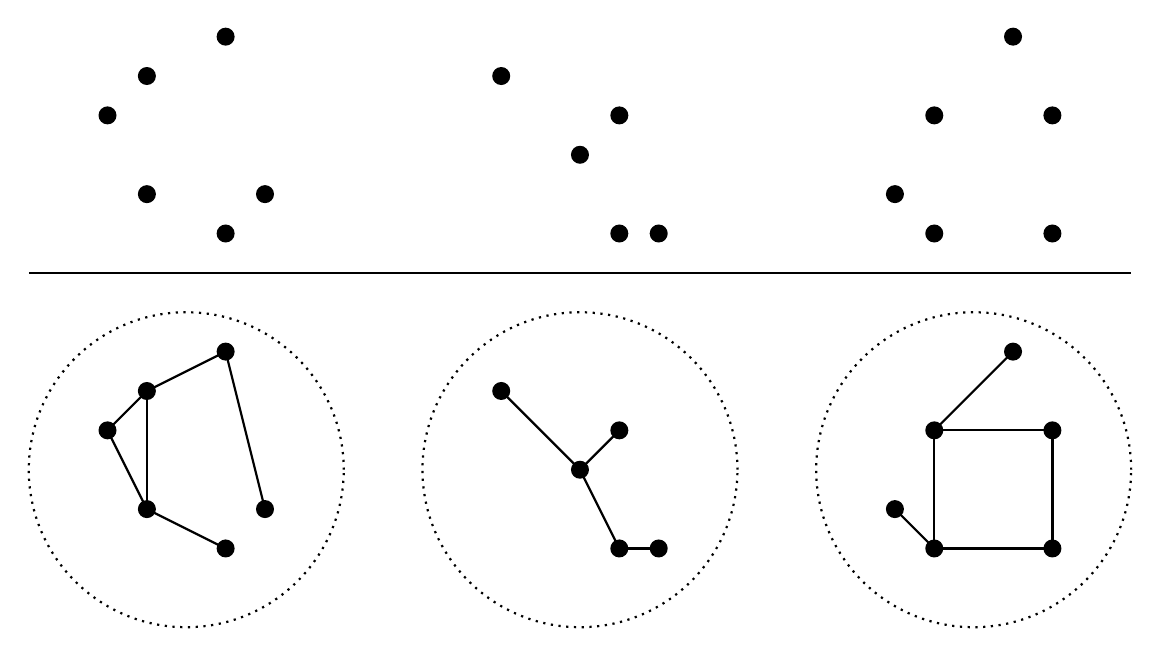
\begin{tikzpicture}

\tikzmath{
\scale = 1;
}

\draw[thick,dotted] (0*\scale,0*\scale) circle(2*\scale);
\draw[thick,fill] (0*\scale,0*\scale) circle(0.1*\scale);
\draw[thick,fill] (0.5*\scale,0.5*\scale) circle(0.1*\scale);
\draw[thick,fill] (-1*\scale,1*\scale) circle(0.1*\scale);
\draw[thick,fill] (0.5*\scale,-1*\scale) circle(0.1*\scale);
\draw[thick,fill] (1*\scale,-1*\scale) circle(0.1*\scale);
\draw[thick] (0*\scale,0*\scale) -- (.5*\scale,.5*\scale);
\draw[thick] (0*\scale,0*\scale) -- (.5*\scale,-1*\scale);
\draw[thick] (.5*\scale,-1*\scale) -- (1*\scale,-1*\scale);
\draw[thick] (0*\scale,0*\scale) -- (-1*\scale,1*\scale);


\draw[thick,dotted] (5*\scale,0*\scale) circle(2*\scale);
\draw[thick,fill] (6*\scale,.5*\scale) circle(0.1*\scale);
\draw[thick,fill] (5.5*\scale,1.5*\scale) circle(0.1*\scale);
\draw[thick,fill] (4.5*\scale,.5*\scale) circle(0.1*\scale);
\draw[thick,fill] (4*\scale,-.5*\scale) circle(0.1*\scale);
\draw[thick,fill] (4.5*\scale,-1*\scale) circle(0.1*\scale);
\draw[thick,fill] (6*\scale,-1*\scale) circle(0.1*\scale);
\draw[thick] (6*\scale,.5*\scale) -- (4.5*\scale,.5*\scale);
\draw[thick] (5.5*\scale,1.5*\scale) -- (4.5*\scale,.5*\scale);
\draw[thick] (6*\scale,-1*\scale) -- (4.5*\scale,-1*\scale);
\draw[thick] (4.5*\scale,-1*\scale) -- (4*\scale,-.5*\scale);
\draw[thick] (4.5*\scale,.5*\scale) -- (4.5*\scale,-1*\scale);
\draw[thick] (6*\scale,-1*\scale) -- (6*\scale,.5*\scale);





\draw[thick,dotted] (-5*\scale,0*\scale) circle(2*\scale);
\draw[thick,fill] (-4.5*\scale,1.5*\scale) circle(0.1*\scale);
\draw[thick,fill] (-5.5*\scale,1*\scale) circle(0.1*\scale);
\draw[thick,fill] (-6*\scale,.5*\scale) circle(0.1*\scale);
\draw[thick,fill] (-5.5*\scale,-.5*\scale) circle(0.1*\scale);
\draw[thick,fill] (-4.5*\scale,-1*\scale) circle(0.1*\scale);
\draw[thick,fill] (-4*\scale,-.5*\scale) circle(0.1*\scale);
\draw[thick] (-4.5*\scale,-1*\scale) -- (-5.5*\scale,-.5*\scale);
\draw[thick] (-5.5*\scale,1*\scale) -- (-5.5*\scale,-.5*\scale);
\draw[thick] (-5.5*\scale,-.5*\scale) -- (-6*\scale,.5*\scale);
\draw[thick] (-6*\scale,.5*\scale) -- (-5.5*\scale,1*\scale);
\draw[thick] (-5.5*\scale,1*\scale) -- (-4.5*\scale,1.5*\scale);
\draw[thick] (-4*\scale,-.5*\scale) -- (-4.5*\scale,1.5*\scale);


\draw[thick] (-7*\scale,2.5*\scale) -- (7*\scale,2.5*\scale);


\draw[thick,fill] (0*\scale,4*\scale) circle(0.1*\scale);
\draw[thick,fill] (0.5*\scale,4.5*\scale) circle(0.1*\scale);
\draw[thick,fill] (-1*\scale,5*\scale) circle(0.1*\scale);
\draw[thick,fill] (0.5*\scale,3*\scale) circle(0.1*\scale);
\draw[thick,fill] (1*\scale,3*\scale) circle(0.1*\scale);




\draw[thick,fill] (6*\scale,4.5*\scale) circle(0.1*\scale);
\draw[thick,fill] (5.5*\scale,5.5*\scale) circle(0.1*\scale);
\draw[thick,fill] (4.5*\scale,4.5*\scale) circle(0.1*\scale);
\draw[thick,fill] (4*\scale,3.5*\scale) circle(0.1*\scale);
\draw[thick,fill] (4.5*\scale,3*\scale) circle(0.1*\scale);
\draw[thick,fill] (6*\scale,3*\scale) circle(0.1*\scale);



\draw[thick,fill] (-4.5*\scale,5.5*\scale) circle(0.1*\scale);
\draw[thick,fill] (-5.5*\scale,5*\scale) circle(0.1*\scale);
\draw[thick,fill] (-6*\scale,4.5*\scale) circle(0.1*\scale);
\draw[thick,fill] (-5.5*\scale,3.5*\scale) circle(0.1*\scale);
\draw[thick,fill] (-4.5*\scale,3*\scale) circle(0.1*\scale);
\draw[thick,fill] (-4*\scale,3.5*\scale) circle(0.1*\scale);




\end{tikzpicture}

\end{center}

\caption{
The program \emph{symbolic\_comparison}
finds particular equivalence relations
that link different identities together,
showing that they belong to the same
equivalence class. In practice,
there are orders of magnitude more
identities (represented as dots) and many more
equivalence classes (the connected subgraphs)
than shown here.
Moreover, the program had access to enough elements
of the group action so that the subgraphs were
usually complete.
}
 
\label{figure_connections}
 
\end{figure}





To show that identities are in the same
equivalence class, the
\emph{symbolic\_comparison}
program
uses particular
group actions from 
$ \mathfrak{S}_4^\pm \times \mathfrak{S}_4^\pm $
to prove equivalence.
An image of this process
appears in 
Figure~\ref{figure_connections}.
This program provides an upper
bound on the number of identities,
but cannot prove that two identities
are not equivalent.

The two programs agree on the values for 
$n = 1$ to $4$. This data appears in 
Table~\ref{table:4D}.


\begin{table}[h]




\begin{center}


\begin{tabular}{ c | c }
 $ n $ & $ \kappa $ \\
\hline\hline
 1 & 1 \\
\hline
 2 & 8 \\
\hline
 3 & 48 \\
\hline
 4 & 965 
\end{tabular}





\end{center}
\caption{
The conjectured number of equivalence
classes $ \kappa $  
in the case where $p = m = 4$.
 }

\label{table:4D}

\end{table}

\newpage



\begin{theorem}
\label{theorem_8_classes}
In the case where  $p = m = 4$ and $n = 2$,
the following identities 
arise from 8 different
equivalence classes.

\begin{align}
\label{Identity_1}
    (x^2 - y^2 - z^2 - w^2 )^2 + (2xy)^2 + (2xz)^2 + (2xw)^2 
    &= (x^2 + y^2 + z^2 + w^2)^2 
\end{align}
\begin{align}
\label{Identity_2}
    (x^2 - y^2 - z^2 + w^2 )^2 + (2xy - 2zw)^2 + (2xz + 2yw)^2 + (0)^2 
    &= (x^2 + y^2 + z^2 + w^2)^2
\end{align}
\begin{align}
\label{Identity_3}
    (x^2 + y^2 + z^2 + w^2 )^2 + (0)^2 + (0)^2 + (0)^2 
    &= (x^2 + y^2 + z^2 + w^2)^2
\end{align}
\begin{align}
\label{Identity_4}
    (x^2 - y^2 - 2zw )^2 + (2xy + z^2 - w^2)^2 
    + (xz - yz + xw + yw)^2\nonumber
    \\
    + (xz - yz + xw + yw)^2 
        &= (x^2 + y^2 + z^2 + w^2)^2
\end{align}
\begin{align}
\label{Identity_5}
    (x^2 - y^2 )^2 + (2xy - z^2 - w^2)^2 
        + (xz + yz + xw + yw)^2 \nonumber
        \\
        + (-xz - yz + xw + yw)^2 
    &= (x^2 + y^2 + z^2 + w^2)^2
\end{align}
\begin{align}
\label{Identity_6}
    (x^2 + y^2 )^2 + (- z^2 - w^2)^2 
        + (xz + yz + xw - yw)^2  \nonumber
        \\
      + (-xz + yz + xw + yw)^2
    &= (x^2 + y^2 + z^2 + w^2)^2
\end{align}
\begin{align}
\label{Identity_7}
    (x^2 - yz - yw - zw )^2 + (xy + xz + yz - w^2)^2 
        + (-y^2 + xz + xw + zw)^2 \nonumber
        \\
        + (xy - z^2 + xw + yw)^2 
    = (x^2 + y^2 + z^2 + w^2)^2
\end{align}
\begin{align}
\label{Identity_8}
    (x^2 - yz + yw - zw )^2 + (xy + xz - yz - w^2)^2 
        + (y^2 + xz + xw + zw)^2 \nonumber
        \\
        + (xw - xy - z^2  + yw)^2 
            = (x^2 + y^2 + z^2 + w^2)^2
\end{align}
Furthermore, each identity
is generated by a product of quaternions. 
\end{theorem}
\begin{proof}
Identity~\eqref{Identity_1} follows from taking the norm of the quaternion product
    \begin{align*}
    (x + iy + jz + kw)(x + iy + jz + kw) 
    = (x^2 - y^2 - z^2 - w^2 ) + i(2xy) + j(2xz) + k(2xw).
    \end{align*}
Identity~\eqref{Identity_2} follows from taking the norm of the quaternion product    
    \begin{align*}
    &(x + iy + jz + kw)(x + iy + jz - kw) \\
    &= (x^2 - y^2 - z^2 + w^2 ) + i(2xy - 2zw) + j(2xz + 2yw) + k(0). 
    \end{align*}
Identity~\eqref{Identity_3} follows from taking the norm of the quaternion product        
    \begin{align*}
    &(x + iy + jz + kw)(x - iy - jz - kw) \\
    &= (x^2 + y^2 + z^2 + w^2 ) + i(0) + j(0) + k(0).
    \end{align*}
Identity~\eqref{Identity_4} follows from taking the norm of the quaternion product        
    \begin{align*}
    &(x + iy + jz + kw)(x + iy + jw + kz) \\
    &= (x^2 - y^2 - 2zw ) + i(2xy + z^2 -w^2) \\
        &+ j(xz - yz + xw + yw) + k(xz - yz + xw + yw).
    \end{align*}
Identity~\eqref{Identity_5} follows from taking the norm of the quaternion product            
    \begin{align*}
    &(x + iy + jz + kw)(x + iy + jw - kz) \\
    &= (x^2 - y^2 ) + i(2xy - z^2 - w^2) \\
        &+ j(xz + yz + xw + yw) + k(-xz - yz + xw + yw).
    \end{align*}
Identity~\eqref{Identity_6} follows from taking the norm of the quaternion product
    \begin{align*}
    &(x + iy + jz + kw)(x - iy + jw - kz) \\
    &= (x^2 + y^2 ) + i(- z^2 - w^2) \\
        &+ j(xz + yz + xw - yw) + k(-xz + yz + xw + yw).
    \end{align*}
Identity~\eqref{Identity_7} follows from taking the norm of the quaternion product
    \begin{align*}
    &(x + iy + jz + kw)(x + iz + jw + ky) \\
    &= (x^2 - yz - yw - zw ) + i(xy + xz + yz - w^2) \\
        &+ j(-y^2 + xz + xw + zw) + k(xy - z^2 + xw + yw).
    \end{align*}
Finally, Identity~\eqref{Identity_8} follows from taking the norm of the quaternion product    
    \begin{align*}
    &(x + iy + jz + kw)(x + iz + jw - ky) \\
    &= (x^2 - yz + yw - zw ) + i(xy + xz - yz - w^2) \\
        &+ j(y^2 + xz + xw + zw) + k(xw - xy - z^2  + yw). \tag*{\qedhere}
    \end{align*}
\end{proof}


\begin{conjecture}
In the case where  $p = m = 4$ and $n = 2$,
there are exactly 8 equivalence classes, which have representatives
given in Theorem~\ref{theorem_8_classes}.
\end{conjecture}

\begin{remark}
The cardinality of each equivalence class in the
set of solutions to $a^2 + b^2 + c^2 + d^2 = (x^2 + y^2 + z^2 + w^2)^2$
can be calculated using the group action under
$ \mathfrak{S}_4^\pm \times \mathfrak{S}_4^\pm $.
The orders of these orbits are, respectively,
$1536$, $1152$, $8$, $2304$, $4608$, $2304$, $3072$, $3072$.
Naturally, all of those numbers are factors of
$ | \mathfrak{S}_4^\pm \times \mathfrak{S}_4^\pm | = 2^{14} 3^2 $.
The programs \emph{numeric\_comparison} and \emph{symbolic\_comparison} 
both used the space of all products of relevant quaternions,
giving a different list of cardinalities:
$4$, $3$, $8$, $6$, $12$, $6$, $8$, $8$.
In fact, the programs were able to ignore large
portions of this space for theoretical reasons,
which is why the cardinalities in this list are
smaller.
In particular, this list represents the number of
nodes in the connected subgraphs found by  \emph{symbolic\_comparison}.
This list is almost the first list
scaled down by a factor of 384, but the third term is inconsistent
for reasons involving conjugates that are discussed more fully in
the proof of Theorem~\ref{theorem_counting_4D}.
\end{remark}

\section{Conjecture for $p = m = 4$ and $ n \in \Nnn $}
The two conjectures in this section were made in collaboration with
Professor David Leep.

We conjecture that when $p = m = 4$ and $ n \in \Nnn $,
all identities of the form
$
\tau_1 ^ 2  + \tau_2 ^ 2  + \tau_3 ^ 2  + \tau_4 ^ 2  
= 
\left(  x_1 ^ 2 + x_2 ^ 2 + x_3 ^ 2 + x_4 ^ 2
\right) ^ n 
$
can be written as
a product of Lipschitz quaternions.
This is made more precise in
Conjecture~\ref{conjecture_Ehrenborg-Leep}.

\begin{conjecture}
Let $ \alpha \in \Lll[x,y,z,w] $.
If the norm $ \N(\alpha) $ has a nontrivial
factorization over $ \Zzz[x,y,z,w] $,
then $ \alpha $ has a nontrivial
factorization over $ \Lll[x,y,z,w] $.
\end{conjecture}
The preceding conjecture implies the following conjecture.
\begin{conjecture}
\label{conjecture_Ehrenborg-Leep}
Let $ (a, b, c, d) $ be a tuple such that
\[
a^2 + b^2 + c^2 + d^2 = (x^2 + y^2 + z^2 + w^2)^n,
\] 
where $ a, b, c, d \in \Zzz[x,y,z,w]$.
Let $\alpha = a + bi + cj + dk $.
Then $ \alpha = \beta_1 \beta_2 \dotsm \beta_n $,
where $ \beta_u \in \Lll[x,y,z,w] $ for $u$ in $1, \dotsc, n$.
Moreover, let $ \beta_u = a' + b'i + c'j + d'k $. Then
the following tuple equivalence holds: $ (a', b', c', d') \simeq (x, y, z, w) $.
\end{conjecture}



\section{Proof of Conjecture~\ref{conjecture_Ehrenborg-Leep} when $n=1$}
I have proved Conjecture~\ref{conjecture_Ehrenborg-Leep}
in the case where $n = 1$.


Recall that $ \theta \in \Zzz[x,y,z,w] $ is a \emph{monomial} if $ \theta $
is of the form $Cx^{e_1}y^{e_2}z^{e_3}w^{e_4}$, where $ C \in \Zzz $
and $ e_1,e_2,e_3,e_4 \in \Nnn \cup \{0\} $.
Two monomials $ u$ and $ v $ are \emph{similar}, denoted  $ u \sim v $,
if they are equal or only differ in their
coefficient.
We denote the degree of  $ \theta $ with respect to the variable $x$ 
by  $\deg_x \theta = e_1 $. We use analogous notation for the
other three variables.

\begin{remark}
Any element of $ \Zzz[x,y,z,w] $ is a sum of monomials.
\end{remark}

\begin{lemma}
If $a, b, c, d \in \Zzz[x,y,z,w]$, and
\[
a^2 + b^2 + c^2 + d^2 = x^2 + y^2 + z^2 + w^2,
\]
then $ (a, b, c, d ) \simeq (x, y, z, w )$.
\end{lemma}
\begin{proof}
Write each of $ a,b,c,d $ as sums of monomials, that is, 
\begin{align*}
&a = \theta_{11} + \theta_{12} + \dotsb + \theta_{1\alpha},
\\
&b = \theta_{21} + \theta_{22} + \dotsb + \theta_{2\beta},
\\
&c = \theta_{31} + \theta_{32} + \dotsb + \theta_{3\gamma},
\\
&d = \theta_{41} + \theta_{42} + \dotsb + \theta_{4\delta},
\end{align*}
where the monomial $ \theta_{ij}$ is not similar
to the monomial $\theta_{ik}$ for $ j \neq k$.

Let $S$ be the \emph{multiset} of all the preceding $ \theta $'s.
We select a particular element~$ \omega $
from $S$ in the following manner.
Let $ S_1 $ be the set of all $ \theta \in S  $ such that
$ \deg_x \theta $ is the maximum possible for all $ \theta \in S $.
Let $ S_2 $ be the set of all $ \theta \in S_1  $ such that
$ \deg_y \theta $ is the maximum possible for all $ \theta \in S_1 $.
Let $ S_3 $ be the set of all $ \theta \in S_2  $ such that
$ \deg_z \theta $ is the maximum possible for all $ \theta \in S_2 $.
Finally, let $ S_4 $ be the set of all $ \theta \in S_3  $ such that
$ \deg_w \theta $ is the maximum possible for all $ \theta \in S_3 $.
Let $ \omega $ be an element of $ S_4 $. 
We can write $ \omega = Cx^{e_1}y^{e_2}z^{e_3}w^{e_4}$, where $ C \in \Zzz $
and $ e_1,e_2,e_3,e_4 \in \Nnn \cup \{0\} $.

We first assume that $\deg_x \omega > 1 $.
In the expression  
$a^2 + b^2 + c^2 + d^2$, there must be at least one monomial similar to $ \omega^2 $
that cancels the term $ \omega^2 = C^2x^{2e_1}y^{2e_2}z^{2e_3}w^{2e_4}$.
Let one of these monomials be $ \psi $. Assume for the moment that $ \psi $
is not formed from squaring a monomial in $S$, but rather
from a product of two nonsimilar monomials.
In other words, $ \psi = \psi' \cdot \psi''$, where $ \psi' \nsim \psi'' $
and $ \psi' , \psi'' \in S $. Since $\omega$ was chosen to have maximal $x$-degree,
we have $\deg_x \psi' \leq \deg_x \omega$ and
$\deg_x \psi'' \leq \deg_x \omega$.
As $\omega^2 \sim \psi = \psi' \cdot \psi''$,
we have $ \deg_x \omega^2 = \deg_x \psi' + \deg_x \psi''$
and immediately have $ \deg_x \omega = \deg_x \psi' = \deg_x \psi'' $.
Thus $ \psi' , \psi'' \in S_1 $. Continuing in this manner
with the other variables, we
conclude that $ \psi' $ and $ \psi'' $ are similar monomials.
This contradicts the fact that $ \psi' \nsim \psi'' $.
Hence $ \psi $ was
formed by the square of a monomial in $ S $. However, this implies the coefficient
of $ \psi $ is positive. Furthermore, the coefficient of
any monomial similar to $ \omega^2 $ must be positive,
so $ \omega^2 $ cannot be cancelled. This is
a contradiction, so $ \deg_x \omega \leq 1 $. Thus no monomial in $S$ has $x$-degree more
than $1$. In an analogous way, we can show that no monomial in $S$ has $y$-degree, $z$-degree,
or $w$-degree more than $1$.

By setting the three variables $y$, $z$, $w$ equal to zero, we see that $ S $ contains
exactly one monomial similar to $ x $, namely $ x$ or $ -x $. The same is true for
the other three variables. Moreover, there are no constants in $ S $.

Assume that $\theta_{11} \sim x$ and $\theta_{12} \sim y$.
Then $a^2$ contains
a monomial similar to $ xy $, which can only be cancelled by another product of monomials similar to
$ x $ and $y$. However, we showed that $ S $ has no such other monomials.
Thus each coordinate $ (a, b, c, d) $ contains exactly one of $ \pm x$, $\pm y$, $\pm z$, $\pm w $.


Assume that the coordinate that contains $ \pm x $ also contains
another monomial $ A = Dx^{f_1}y^{f_2}z^{f_3}w^{f_4}$, where $ D \in \Zzz $
and $ f_1,f_2,f_3,f_4 \in \{0,1\} $. Then $ A^2 $ has degrees (with respect to
each variable) of either 0 or 2. To cancel $ A^2 $, we must find a product of two
monomials in $ S $ that is similar to $ A^2 $. As no monomial in $ S $ has a degree
(with respect to any variable) of two, any monomial similar to $ A^2 $ must itself be
a square of a monomial similar to $ A $. In this case, the coefficients are
positive and will not cancel. Thus there can be no such monomial~$ A $, so the only monomials
in $ S $ are the four desired ones.
\end{proof}

\section{Enumerative Consequences of Conjecture~\ref{conjecture_Ehrenborg-Leep}} 

\begin{theorem}
\label{theorem_counting_4D}
Assuming Conjecture~\ref{conjecture_Ehrenborg-Leep} holds,
then the number of solutions $ (a, b, c, d) $ to
\begin{equation}
\label{equation_4D}
a^2 + b^2 + c^2 + d^2 = (x^2 + y^2 + z^2 + w^2)^n,
\end{equation}
where $ a, b, c, d \in \Zzz[x,y,z,w]$,
is at most
\[
8 \cdot \frac{47^{n+1} - 1}{46}
=  8 \cdot \left\lfloor \frac{ 47^{n+1} }{46} \right\rfloor
=  8 \sum_{i = 0}^n{47^n}.
\]
\end{theorem}
\begin{proof}
If Conjecture~\ref{conjecture_Ehrenborg-Leep} holds, any
solution
$ (a, b, c, d) $ can be viewed as a quaternion
$ a + bi + cj + dk = \beta_1 \beta_2 \dotsm \beta_n $
where the $\beta_i$ are quaternions from the following set:
\[
T_1 = \{ \pm a' \pm b'i \pm c'j \pm d'k
\text{ : } \{ a', b', c', d' \} = \{ x, y, z, w \} \}. 
\]
Note that $ | T_1 | = 2^4 4! = 384 $.
Thus there are at most $ 384^n $ unique solutions to equation~\eqref{equation_4D}.
Using the fact that
\[
\beta_1 \beta_2 \dotsm \beta_i \beta_{i+1} \dotsm \beta_n
=
\beta_1 \beta_2 \dotsm \beta_i u u^{-1} \beta_{i+1} \dotsm \beta_n,
\]
where $ u \in \{ \pm 1 , \pm i, \pm j, \pm k \} $ is a unit of $\Lll$,
we can specify
that every $\beta_i$ except the first has $ a' = x $ without
losing any solutions. Thus the number of unique solutions
to equation~\eqref{equation_4D} is at most
$ 384 \cdot 48^{n-1} $. Alternatively, we can factor out a unit
from the first factor $\beta_1$ to ensure that it has $ a' = x $, so the
resulting product is of the form $ u \beta_1 \beta_2 \dotsm \beta_n $,
where each $ \beta_i $ belongs to
\[
T_2 = \{ x \pm b'i \pm c'j \pm d'k
\text{ : } \{ b', c', d' \} = \{ y, z, w \} \},
\]
with $ | T_2 | = 2^3 3! = 48 $.

If any two consecutive $ \beta $'s are conjugates, we can combine them
to form $ x^2 + y^2 + z^2 + w^2 $. As this is a real number, we can
factor it out. The product is now of the form
\[
(x^2 + y^2 + z^2 + w^2)^\gamma u \beta_1 \beta_2 \dotsm \beta_{n-2\gamma},
\]
with $ \gamma $ ranging over $ 0, 1, \dotsc, \left\lfloor \myfrac{n}{2} \right\rfloor $.

Assume $ n $ is even.
When $ \gamma = \myfrac{n}{2} $, the product is of the form
$ (x^2 + y^2 + z^2 + w^2)^{\myfrac{n}{2}} u  $, so there are 8 unique values, one for
each unit.
When $ \gamma = \myfrac{n}{2} - 1 $, the product is of the form
$ (x^2 + y^2 + z^2 + w^2)^{\myfrac{n}{2} - 1} u \beta_1 \beta_2  $. Although $ \beta_1 $
can be any element of $ T_2 $, $ \beta_2 $ cannot be equal to $ \overline{ \beta_1 } $,
so the number of solutions in this case is $ 8 \cdot 48 \cdot 47 $. The same restriction
applies for all $ \gamma < \myfrac{n}{2} $. For $ \gamma < \myfrac{n}{2} $,
the number of
solutions is $ 8 \cdot 48 \cdot 47^{n - 2\gamma - 1} $.
Summing over all possible values of $ \gamma $, the number of solutions is
\begin{align*}
8 + 8 \cdot 48 \cdot 47 + 8 \cdot 48 \cdot 47^3 + \dotsb
+ 8 \cdot 48 \cdot 47^{n-1}
&= 8 + 8 \cdot 48 \cdot 47 \cdot \frac{47^{2 \cdot \myfrac{n}{2} } - 1 }{47^2 - 1}
\\
&= 8 + 8 \cdot 47 \cdot \frac{47^{n} - 1 }{47 - 1}
\\
&= 8 \left(1 +  \frac{47 (47^{n} - 1 ) }{46}\right)
\\
&= 8 \left( \frac{46 + (47^{n+1} - 47 ) }{46}\right)
\\
&= 8 \left( \frac{47^{n+1} -1 }{46}\right).
\end{align*}

Now assume $ n $ is odd.
When $ \gamma = \myfrac{(n-1)}{2} $, the product is of the form
$ (x^2 + y^2 + z^2 + w^2)^{\myfrac{(n-1)}{2}} u \beta_1  $, so there are $ 8 \cdot 48 $
unique solutions.
When $ \gamma = \myfrac{(n-1)}{2} - 1 = \myfrac{(n-3)}{2}  $, the product is of the form
$ (x^2 + y^2 + z^2 + w^2)^{\myfrac{(n-3)}{2}} u \beta_1 \beta_2 \beta_3  $. Although $ \beta_1 $
can be any element of $ T_2 $, $ \beta_2 \neq \overline{ \beta_1 } $
and $ \beta_3 \neq \overline{ \beta_2 } $,
so the number of solutions in this case is $ 8 \cdot 48 \cdot 47^2 $. The same restriction
applies for all $ \gamma < \myfrac{(n-1)}{2} $. For $ \gamma < \myfrac{(n-1)}{2} $,
the number of solutions is $ 8 \cdot 48 \cdot 47^{n - 2\gamma - 1 } $.
Summing over all values of $ \gamma $, the number of solutions is
\begin{align*}
8 \cdot 48 + 8 \cdot 48 \cdot 47^2 + 8 \cdot 48 \cdot 47^4 + \dotsb
+ 8 \cdot 48 \cdot 47^{n-1}
&= 8 \cdot 48 \cdot \frac{47^{2 \cdot \myfrac{(n+1)}{2} } - 1 }{47^2 - 1}
\\
&= 8  \cdot \frac{47^{n+1} - 1 }{47 - 1}. \qedhere
\end{align*}
\end{proof}
\begin{remark}
Note that the proof of Theorem~\ref{theorem_counting_4D}
gives an upper bound for the number of solutions.
\end{remark}




\section{Conclusion}



This paper is a significant advance
over the author's previous
estimate 
in~\cite{Ehrenborg_2018}
of the number of equivalence classes
when
$p = m = 4$ and $n=2$. Using the two
new computational methods discussed
in Section~\ref{sec:4D}, the upper bound
has been reduced from $57$ to $8$,
assuming Conjecture~\ref{conjecture_Ehrenborg-Leep}
holds.

It is notable that the number of solutions
when $p = m = 2$ increases linearly in
$n$, but the number of solutions
when $p = m = 4$
is asymptotic to an
exponential
function
in $n$.

Future steps include the following:
\begin{enumerate}
\item A proof of
Conjecture~\ref{conjecture_Ehrenborg-Leep}
would solidify Theorem~\ref{theorem_counting_4D}
and provide more theoretical insight
into the nature of these identities.
\item Experimental data shows that 
Theorem~\ref{theorem_counting_4D}
gives the exact number of solutions
in the cases where $n = 0, 1, 2, 3$.
This data was collected by applying the
group action of
$ \mathfrak{S}_4^\pm \times \mathfrak{S}_4^\pm $
to a representative from each equivalence
class and counting the unique identities.
It seems plausible that for all $n$
the expression  $ 8 \sum_{i = 0}^n{47^n} $ is
a lower bound as well as an upper bound.
\item It is difficult to approach the equation
$ \sum_{j = 1}^{p} \tau_j ^ 2 = \left( \sum_{i = 1}^{m} x_i ^ 2 \right) ^ n $
in cases besides $p = m = 2$ and $p = m = 4$, since
the only division rings with a norm are the reals, the complex
numbers, the quaternions, and the $8$-dimensional
octonions, as was proven by Hurwitz in~\cite{Hurwitz}.
I may be able to approach the case $p = m = 8$
using the octonions,
although the lack of associativity presents
new challenges.
Alternatively, I may be able to adapt
the proof of Theorem~\ref{theorem_counting_4D} to
cases when $p$ and $m$ take on values
less than four.
\end{enumerate}

%\newpage

\newcommand{\journal}[6]{{\sc #1,} #2, {\it #3} {\bf #4} (#5), #6.}
\newcommand{\preprint}[3]{{\sc #1,} #2, preprint #3.}
\newcommand{\book}[4]{{\sc #1,} #2, #3, #4.}
\newcommand{\collection}[6]{{\sc #1,}  #2, #3, in {\it #4}, #5, #6.}
\newcommand{\JCTA}{J.\ Combin.\ Theory Ser.\ A}
\newcommand{\arxiv}[3]{{\sc #1,} #2, {\tt #3}.}
\newcommand{\article}[3]{{\sc #1,} #2, {\tt #3}.}






\begin{thebibliography}{1}



\bibitem{Baez}
\journal{J.\ C.\ Baez}
        {Review of ``On Quaternions and Octonions: 
         Their Geometry, Arithmetic and Symmetry''}
        {Bull.\ Amer.\ Math.\ Soc.}{42}{2005}{229--243}
        


\bibitem{Barning}
\journal{F.\  J.\  M.\  Barning} 
      {On Pythagorean and quasi-Pythagorean triangles and a
      generation process with the help of unimodular matrices (Dutch)}
      {Math.\ Centrum Amsterdam Afd.\ Zuivere Wisk.}
      {ZW-011}{1963}{37 pp}



\bibitem{Berggren}
\journal{B.\ Berggren} 
        {Pytagoreiska trianglar (Swedish)} 
        {Elementa: Tidskrift f\"or element\"ar
        matematik, fysik och kemi.}
        {17}{1934}{129--139}

\bibitem{Conrad}
\journal{K.\ Conrad}
        {Pythagorean descent}
        {}
        {}{Preprint}{1-9}



\bibitem{Conway_and_Smith}
\book{J.\ Conway and D.\ Smith}
     {On Quaternions and Octonions: 
      Their Geometry, Arithmetic and Symmetry}
     {A K Peters, Ltd., Natick MA}
     {2003}


\bibitem{Davidoff_Sarnak_Valette}
\book{G.\ Davidoff, P.\ Sarnak, and A.\ Valette}
         {Elementary Number Theory,
           Group Theory,
           and Ramanujan Graphs}
         {Cambridge University Press}
         {2003}

\bibitem{Dickson}
\book{L.\ E.\ Dickson}
         {History of the Theory of Numbers}
         {AMS Chelsea Publishing}
         {1999}

\bibitem{Ehrenborg_2018}
\preprint{T.\ Ehrenborg}
        {Pythagorean Quintuples and Quaternions}
        {2018}




\bibitem{Ferrari}
\journal{F.\ Ferrari}
        {Risoluzione Dell'Equazione}
        {Supplemento al Periodico di Matematica}
        {11}{1908}{129--131}



\bibitem{Frisch_and_Vaserstein}
\journal{S.\ Frisch and L.\ Vaserstein}
       {Polynomial parametrization of Pythagorean quadruples,
        quintuples and sextuples}
       {J.\ Pure Appl.\ Algebra}{216}{2012}{184--191}


\bibitem{Guzeltepe}
\journal{M.\ G\"uzeltepe}
        {Codes over Hurwitz integers}
        {Discrete Math.}
        {313}{2013}{704--714}



\bibitem{Halai}
\article{C.\ Halai}
      {Triples and Quadruples: From Pythagoras to Fermat}
      {plus.maths.org/ content/triples-and-quadruples}{}

\bibitem{Hamilton}
\journal{W.\ Hamilton}
        {On Quaternions; or on a new System of Imaginaries in Algebra}
        {The London, Edinburgh and Dublin Philosophical Magazine
         and Journal of Science}
        {25}{1844}{10--13}


\bibitem{Hardy_and_Wright}
\book{G.\ H.\ Hardy and E.\ M.\ Wright}
         {An Introduction to the Theory of Numbers, 6th Edition}
         {Oxford University Press, Oxford} 
         {2008}




\bibitem{Hatcher}
\book{A.\ Hatcher}
         {Topology of Numbers}
         {Manuscript}
         {February 2018 version}



\bibitem{Heath}
\book{T.\ L.\ Heath}
     {Diophantus of Alexandria, 2nd Edition}
     {Cambridge University Press, London}
     {1910}


\bibitem{Hurwitz}
\journal{A.\ Hurwitz}
        {\"Uber die Komposition der quadratischen Formen}
        {Mathematische Annalen}
        {88}{1922}{1--25}

\bibitem{Jacobi}
\journal{C.\ G.\ J.\ Jacobi}
        {De compositione numerorum e quatuor quadratis}
        {Journal f\"ur die reine und angewandte Mathematik}
        {12}{1834}{167--172}

\bibitem{Euclid}
\article{D.\ E.\ Joyce}
        {Euclid's Elements, Book X, Proposition 29}
        {\\https://mathcs.clarku.edu/\~{}djoyce/java/elements/elements.html}



\bibitem{Lalin}
\article{M.\ N.\ Lal\'in}
      {Every Positive Integer is the Sum of Four Squares! (and other
      exciting problems)} 
      {Sophex –-- University of Texas at Austin, 6
      pp}{}

\bibitem{Mordell}
\book{L.\ J.\ Mordell}
         {Diophantine Equations}
         {Academic Press, London and New York} 
         {1969}




\bibitem{Roy_and_Sonia}
\arxiv{T.\ Roy and F.\ J.\ Sonia}
      {A direct method to generate Pythagorean triples and its
       generalization to Pythagorean quadruples and $n$-tuples}
      {arXiv:1201.2145 [math.NT], 11 pp}



\end{thebibliography}





\end{document}










